\documentclass{article}

% Margins
\usepackage[top=2.5cm, left=3cm, right=3cm, bottom=4.0cm]{geometry}
\geometry{legalpaper, portrait, margin=1.25in}
\usepackage[english]{babel}
\usepackage[utf8]{inputenc}
\usepackage{amsmath,amssymb}
\usepackage{parskip}
\usepackage{graphicx}
\usepackage{placeins}

% Colour table cells
% \usepackage[table]{xcolor}

% Get larger line spacing in table
\newcommand{\tablespace}{\\[1.25mm]}
\newcommand\Tstrut{\rule{0pt}{2.6ex}}         % = `top' strut
\newcommand\tstrut{\rule{0pt}{2.0ex}}         % = `top' strut
\newcommand\Bstrut{\rule[-0.9ex]{0pt}{0pt}}   % = `bottom' strut

%%%%%%%%%%%%%%%%%
%     Title     %
%%%%%%%%%%%%%%%%%
\title{\vspace{-30}Statistical Programming for Social Data Science\\Coursework 1\\Analysis of the relationship between ESG markers, GDP and $CO_2$ emissions}
\author{Candidate Number: BBLF1\\Student Number: 22232992}
\date{\vspace{-10}\today}

\begin{document}
	\maketitle
	\section{Introduction}
	The following report analyzes the relation between the ESG indicators and the GDP with the $CO_2$ emissions of 191 countries around the world.
	Particularly, this paper is aimed at testing the hypothesis where lower GDP values lead to lower $CO_2$ emissions per capita, but higher $CO_2$ emissions per Watt. Moreover, we want to analyze the relationship between other ESG indicators (e.g. gender equity, fair distribution of well-being, government expenditure on education, control of corruption, political stability) lead to higher $CO_2$ emissions per capita.
	- gender equity
	- access to the Internet
	- government expenditure on education
	- control of corruption
	- political stability
	
	\section{Datasets}
	\subsection{ESG dataset}
	The World Bank’s ESG Data Draft dataset (ESG\_dataset) provides information on 17 key sustainability themes spanning environmental, social, and governance categories for 239 countries. For each country, the dataset describes the trend over time of 67 ESG indicators and each ESG marker has been evaluated for the years from 1960 to 2021. 
	Even though the dataset contains the whole time-series of the ESG indicators over time, I decided to select only one specific year because I have not taken a proper course for time-series analysis yet. 

	\subsubsection{Selecting the Year and the ESG indicators} \label{sec:selecting_year_esg}
	The dataset contains many ESG indicators and many years, but we are only interested in one year and 5-10 ESG indicators as covariates. Moreover, most of the ESG indicators and years analyzed contain many missing values, so we analyzed the distribution of NAs in order to find the year with the lowest number of missing values in the relevant ESG indicators.
	
	The biggest challenge is that the number of missing values in the selected year depends on the subset of ESG indicator selected, and the number of missing values of the ESG indicators depends on the selected year. To solve this, we selected them in three steps.
	
	\paragraph{Step 1: Select a large subset of relevant ESG indicators}
	As the first step, we selected a subset (\textit{list1}) of 29 ESG indicators (2-3 similar indicators for each covariate that we would like to consider), that will enable us to compute the missing values for each year while considering only the relevant markers.
	
	
	\paragraph{Step 2: Select the Year}
	Relatively to the year selection, the idea is to select the most recent year with the lowest number of missing values, when considering only the relevant ESG indicators, previously selected in step 1.
	The Figure ~\ref{fig:nan_per_year_and_indicator} shows the barplot that displays how many missing values in the relevant ESG markers are associated with each year, along with the trend of two of the relevant markers.
	Based on the plot, we identified 2018 as the most convenient year.
	
	\begin{figure} [th] 
		\centering
		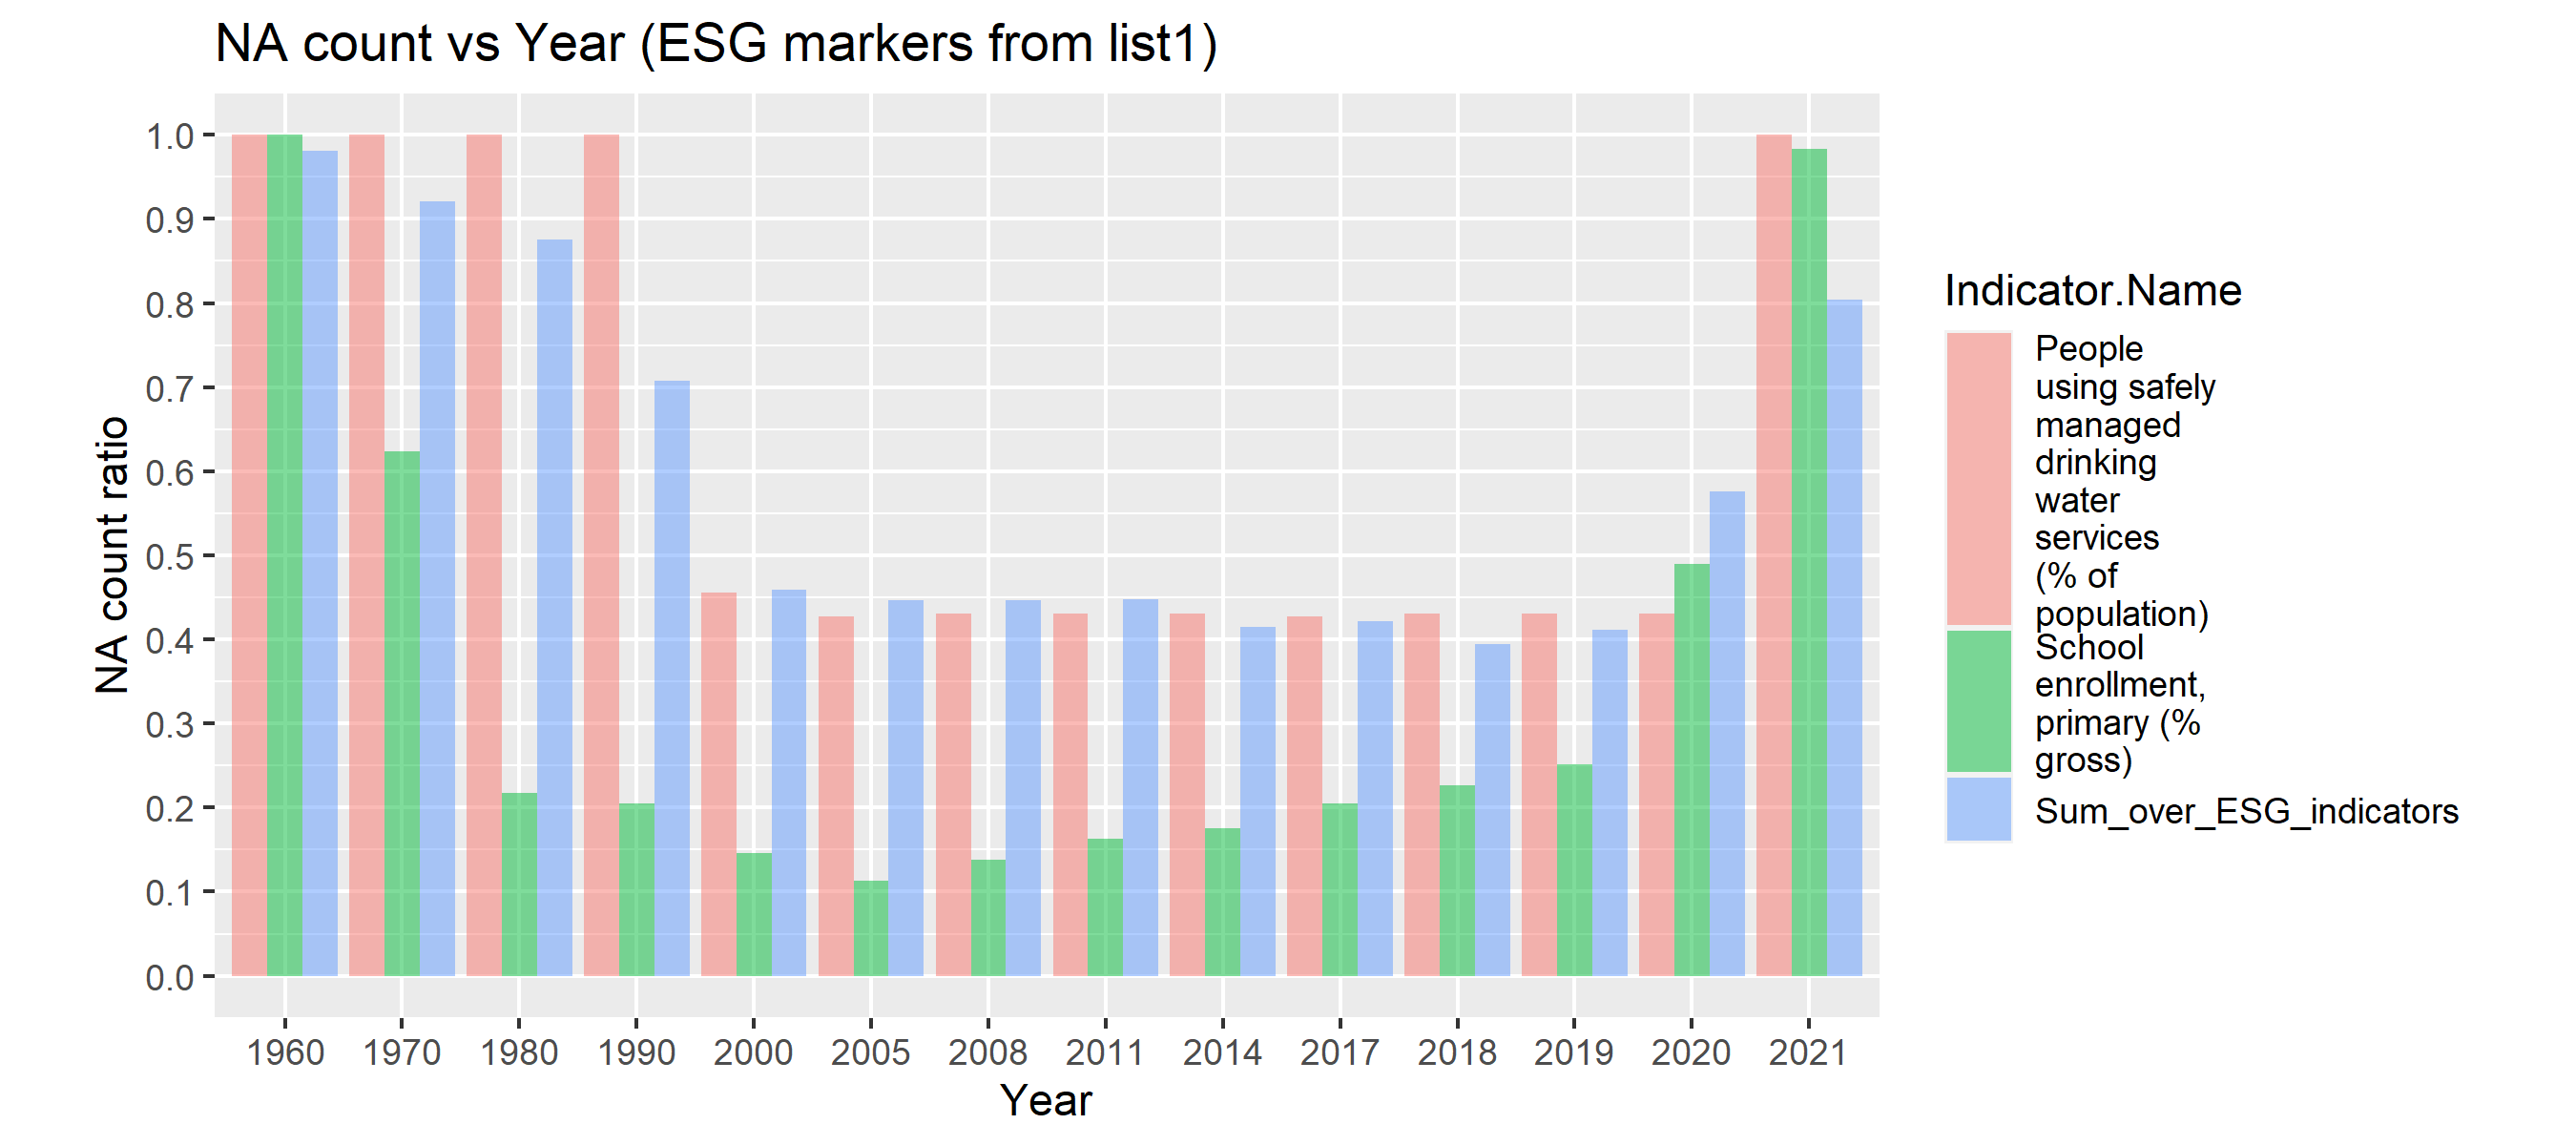
\includegraphics[width=1\linewidth]{nan_per_year_and_indicator.png}
		\caption{\textit{Plot showing the count of missing values in a subset of ESG markers over the years 1960-2021. Particularly, the \textbf{Sum\_over\_ESG\_indicators} serie considers the total count of missing values in the most relevant subset of ESG indicators (list\_1). Notice that the ticks of the x-axis are not equally distant years, to improve readability and to focus the attention on the more recent years, which contain the lowest count of missing values. }}
		\label{fig:nan_per_year_and_indicator}
	\end{figure}
	
	\begin{figure} 
		\centering
		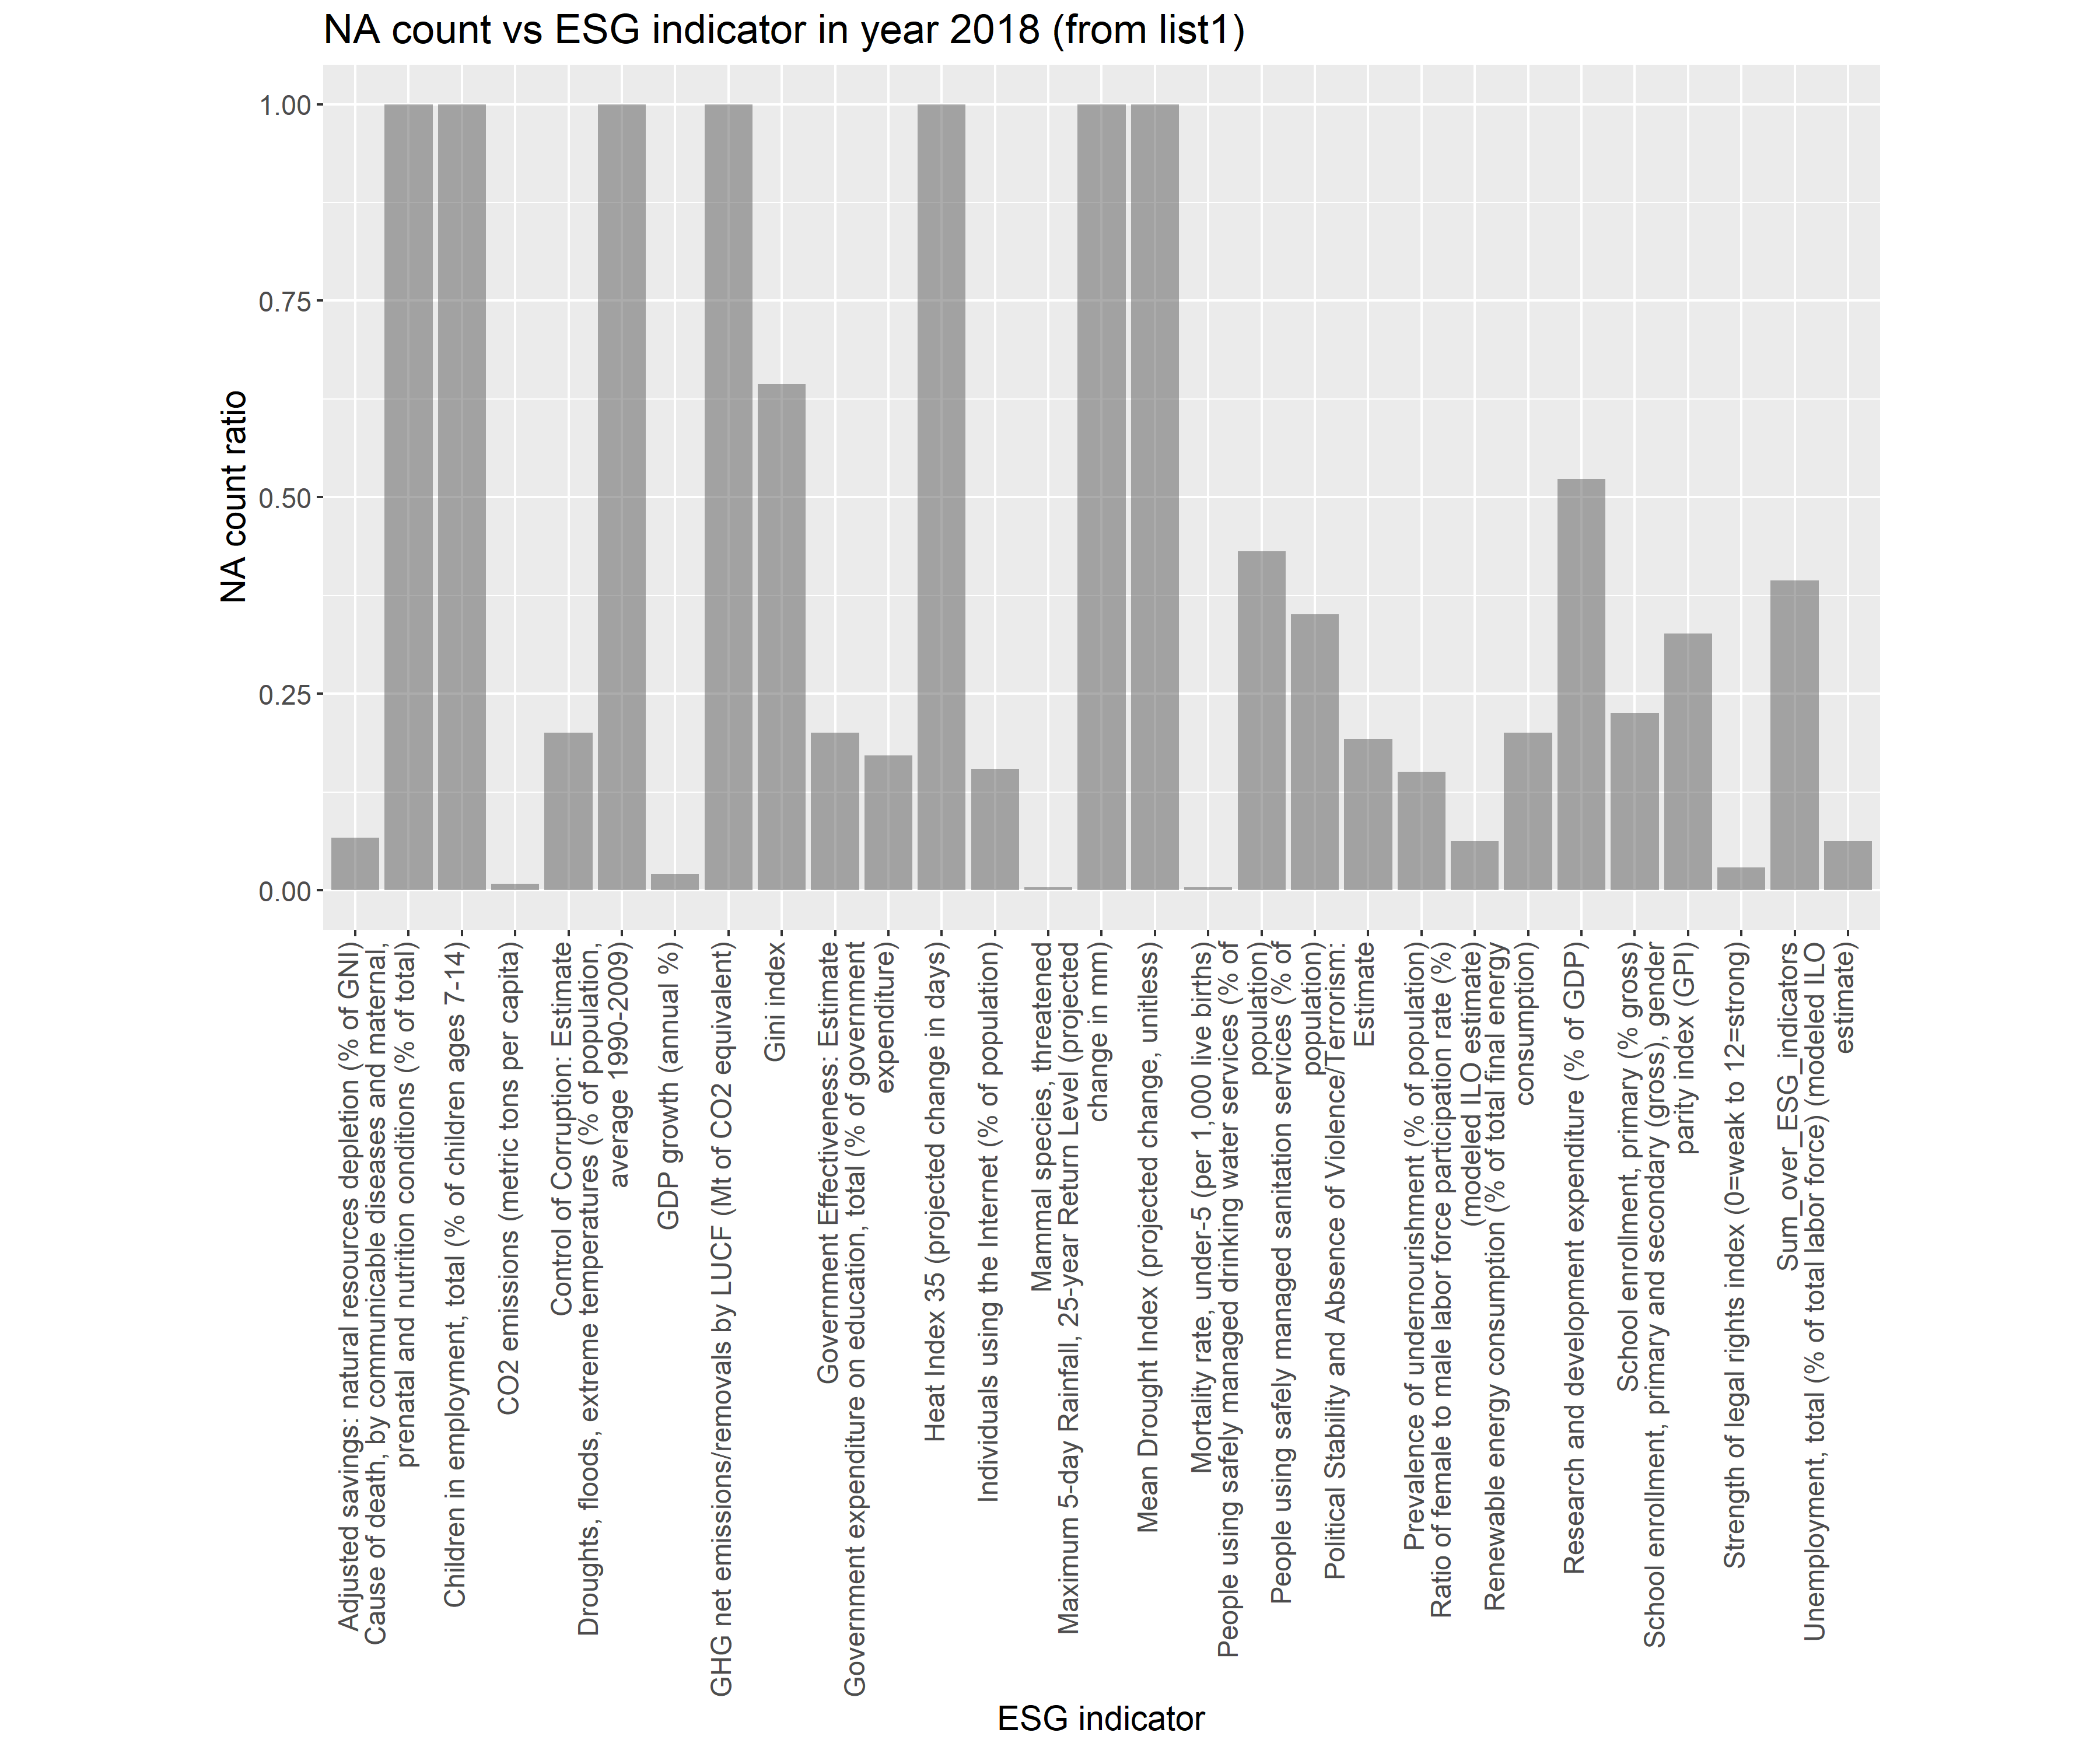
\includegraphics[width=1\linewidth]{nan_2018_per_esg_indicator.png}
		\caption{\textit{Plot showing the count of missing values in the large subset of ESG markers (list1) when considering the year 2018 only.}}
		\label{fig:nan_2018_per_esg_indicator}
	\end{figure}
	\begin{figure} 
		\centering
		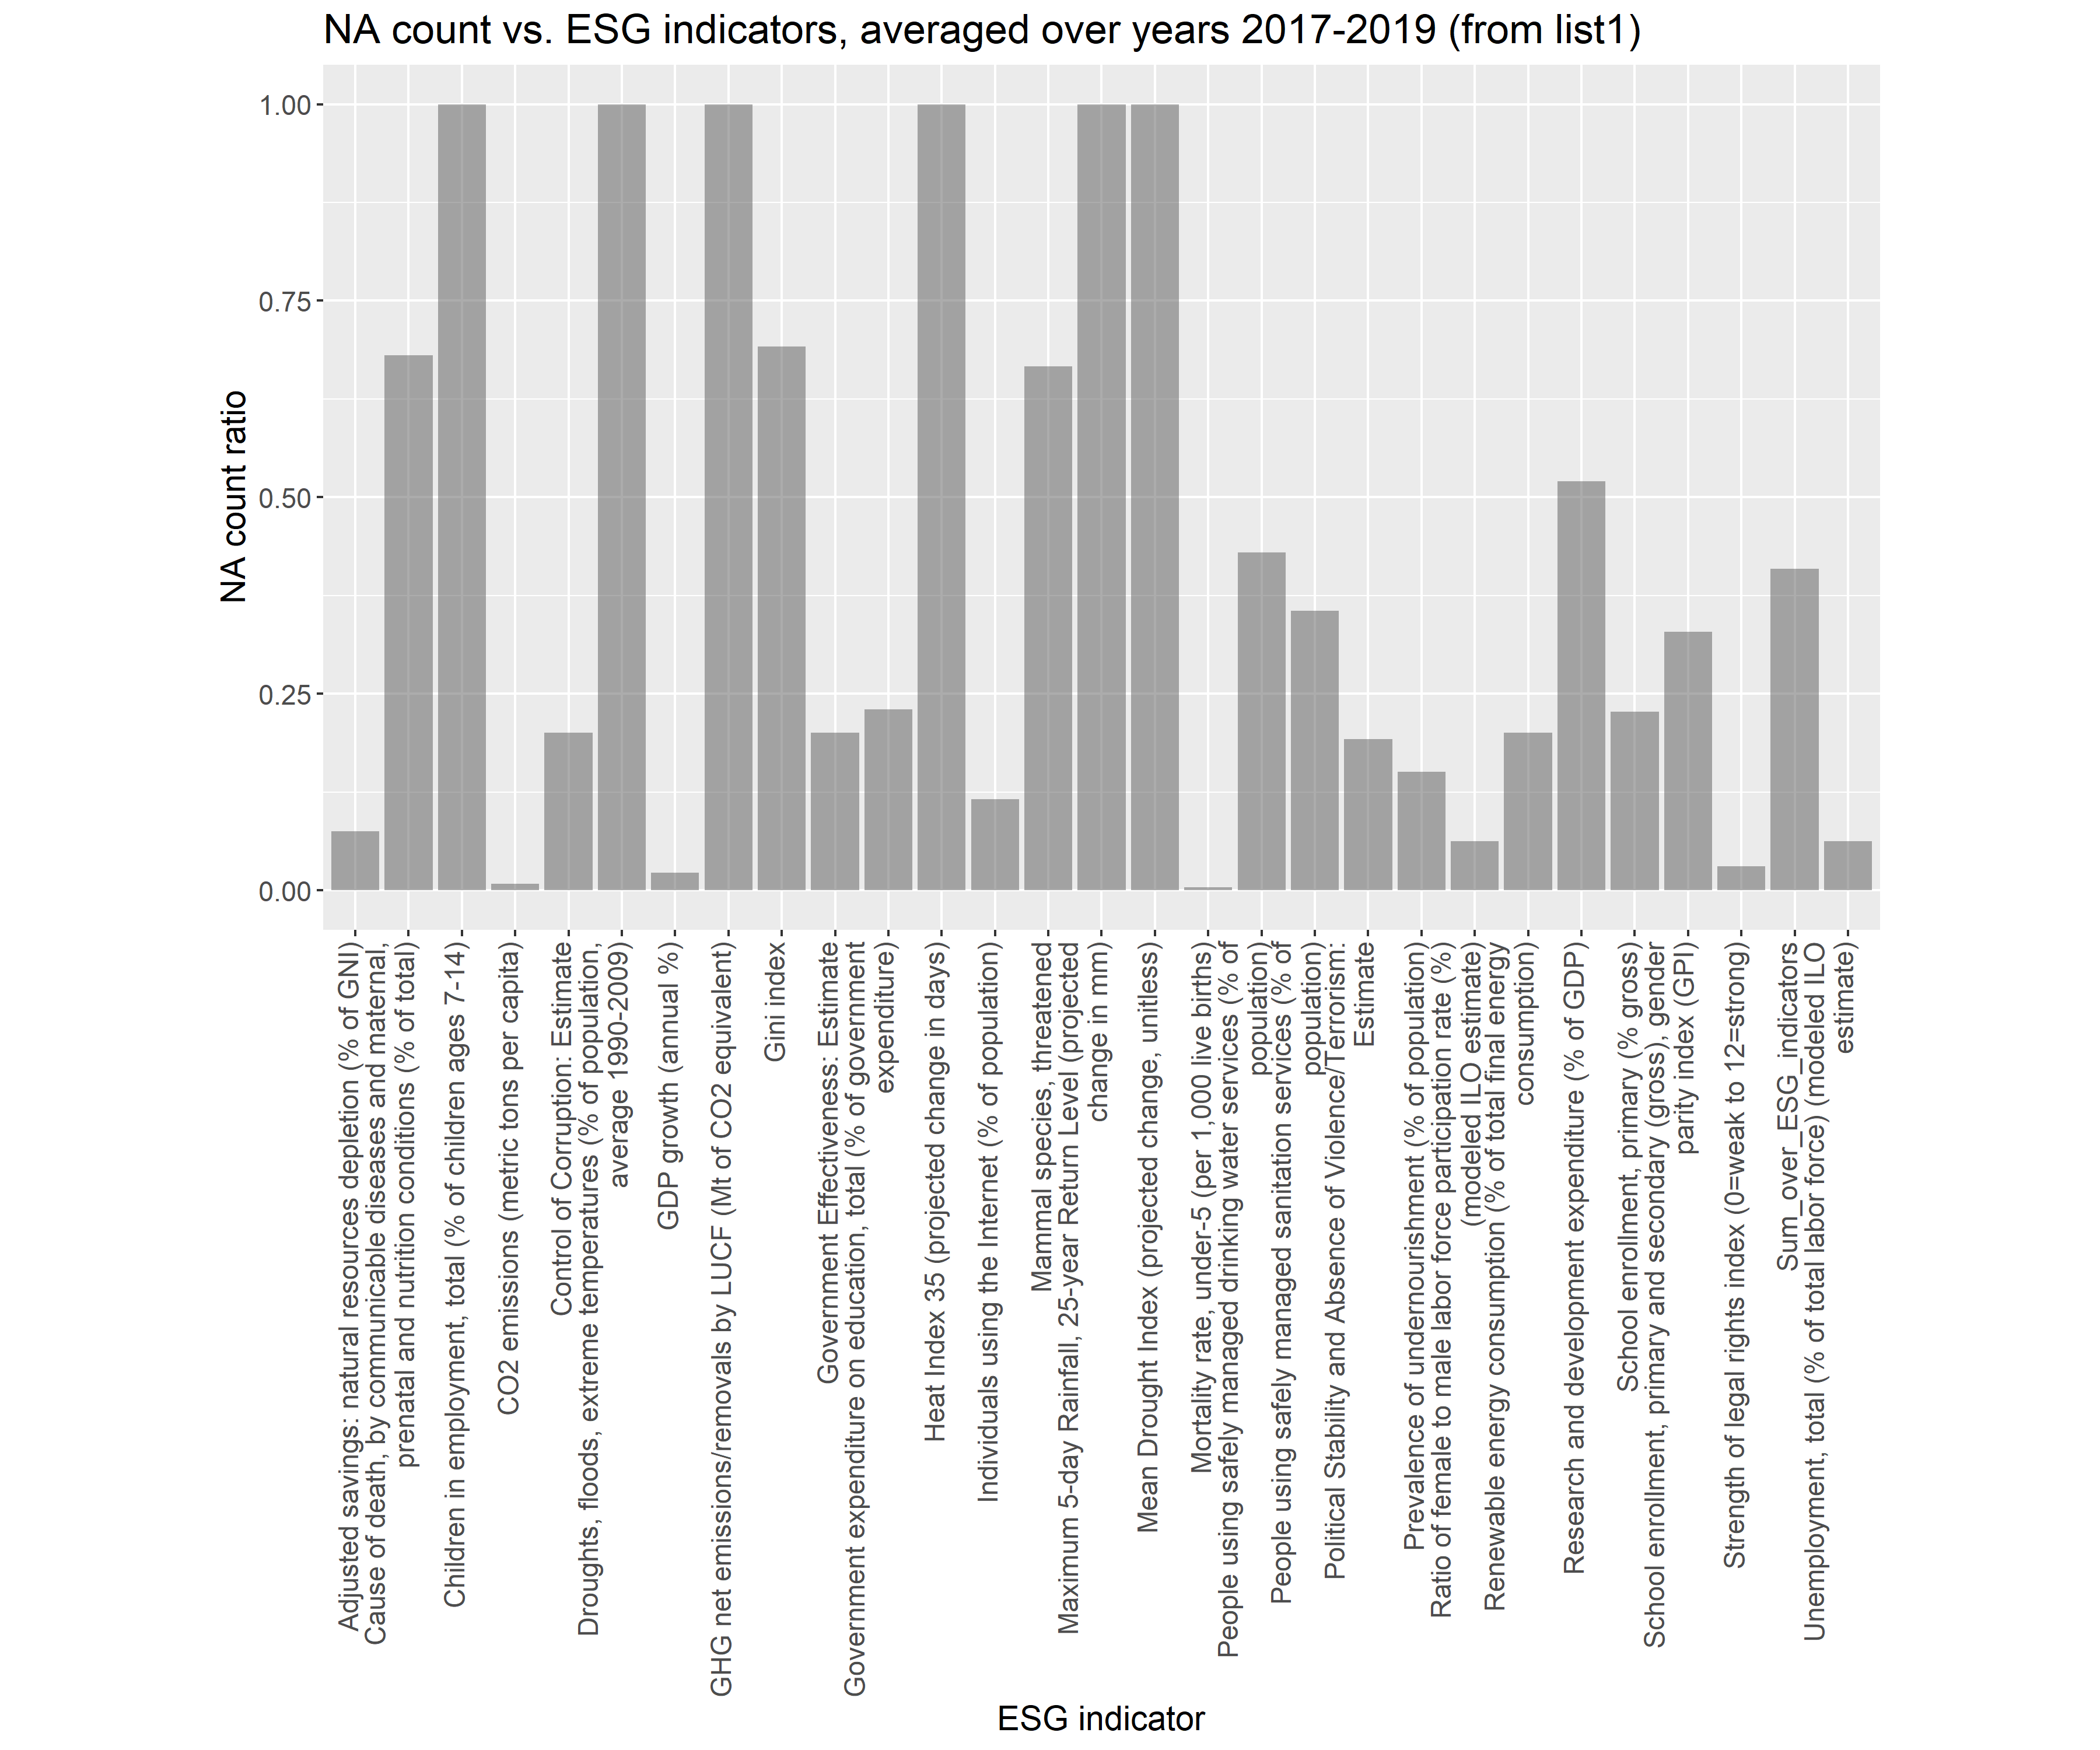
\includegraphics[width=1\linewidth]{nan_mean_2018_per_esg_indicator.png}
		\caption{\textit{Plot showing the count of missing values in a large subset of ESG markers (list1) when considering the average over the years 2017-2019. This is meant to reduce the missing value count by considering the nearest neighbours of the year 2018, when there is a missing value in 2018.}}
		\label{fig:nan_mean_2018_per_esg_indicator}
	\end{figure}

	\paragraph{Step 3: Select a small subset of ESG indicators}
	After selecting the year, we analyzed the large subset of ESG markers  considering:
	\begin{enumerate}
		\item the missing values of each indicator in year 2018 only (see Figure ~\ref{fig:nan_2018_per_esg_indicator})
		\item the missing values of each indicator when considering the mean of the years 2017-2019 (while temporarily removing NAs in the computation). This is supposed to reduce the count of missing values, but, according to Figure ~\ref{fig:nan_mean_2018_per_esg_indicator}, this approach does not show a significant improvement over 1.
	\end{enumerate}
	
	Therefore, we selected the best ESG indicators, based on these results and on the following criteria:
	\begin{itemize}
		\item count of missing values in year 2018
		\item relevance in relation to $CO_2\ emission$ outcome variable
		\item non-multiple collinearity with the other ESG indicators selected.
	\end{itemize}
	
	Finally the selected small subset of ESG indicators (\textit{list2}) is found in Table ~\ref{table:esg_small_set} 
	
	\begin{table}
		\centering
		\begin{tabular}{|c|p{7cm}|p{5cm}|}
			\cline{1-3}
			Category & ESG indicator & \\
			\hline \hline
			Economy & Adjusted savings: natural resources depletion (\% of GNI) & Natural resource depletion is the sum of net forest depletion, energy depletion, and mineral depletion\\
			& Individuals using the Internet (\% of population) & \\
			\hline
			& Government Effectiveness: Estimate & \\
			Governance & Government expenditure on education, total (\% of government expenditure) & \\
			& Control of Corruption: Estimate & \\
			\hline
			Human Rights & Ratio of female to male labor force participation rate (\%) (modeled ILO estimate) & \\
			\hline
			Social and Health & Mortality rate, under-5 (per 1,000 live births) & \\
			& School enrollment, primary (\% gross) & \\
			\cline{1-3}
		\end{tabular}
		\caption{\textit{Table describing the ESG markers selected and their category}}
		\label{table:esg_small_set}
	\end{table}

	\subsubsection{Cleaning the ESG dataset}
	To clean the ESG dataset we performed the following steps:
	\begin{enumerate}
		\item Drop the ``Indicator.Code`` column (we do not need a standardized code for it)
		\item Fix the names of the Year columns by removing the initial ``X`` character
		\item Analyze the ESG indicators contained in the dataset and select the most convenient ones as described in Section ~\ref{sec:selecting_year_esg}.
		\item Drop the remaining missing values
	\end{enumerate}

	\subsection{CO2 emission dataset}
	The second dataset has been created by \textit{Our World in Data}, a project of the Global Change Data Lab, which is a non-profit organization based in the United Kingdom.
	The data is built upon a number of datasets and processing steps, like the \textit{Statistical review of world energy} from the BP company for the $CO_2$ emissions by energy type and the \textit{Climate Adaptation Integration Tool (CAIT)} from World Resources Institute for the GHG emissions.
	
	\subsubsection{Cleaning the CO2 emission dataset}
	To clean the $CO_2$ dataset we followed the steps:
	\begin{enumerate}
		\item Filter on the Year column based on the same year 2018 selected for the \textit{ESG\_dataset}, and then drop the ``year`` column
		\item Filter the Country codes, based on the ones available in the ESG dataset
		\item Compute the ratio of NAs for each covariate. 	According to the results, there are no NAs in the CO2 dataset, except 
		for 5\% in \textit{gdp} column and 19\% in \textit{trade\_co2} of missing values.
		For this reason, we decided to use only the columns \textit{gdp}, \textit{co2\_per\_capita}, and \textit{total\_ghg}.
		\item Based on previous results, we drop \textit{trade\_co2} column and we drop NAs from \textit{gdp} column:
	\end{enumerate}
	
	\section{Merging Datasets based on country codes}
	In order to merge the 2 datasets, we use the standardized country codes. Out of the original 191 common countries, we only have 95 countries, shared between the datasets, after filtering out the rows with NAs.
	
	\subsection{Cleaning merged dataset}
	To clean the resuting \textit{merged dataset} we followed the steps:
	\begin{enumerate}
		\item Renaming the columns containing the country names in order to distinguish the original dataset and verify possible name incoherences
		\item Compute the greenhouse gases emission values per capita by applying the following equation for each row:
		\begin{equation}
			value\ pro\ capita \backsim \frac{absolute\ value}{population}
		\end{equation}
	\end{enumerate}
	
	\subsection{Plotting the distribution of the OLS covariates}
	\begin{figure}
		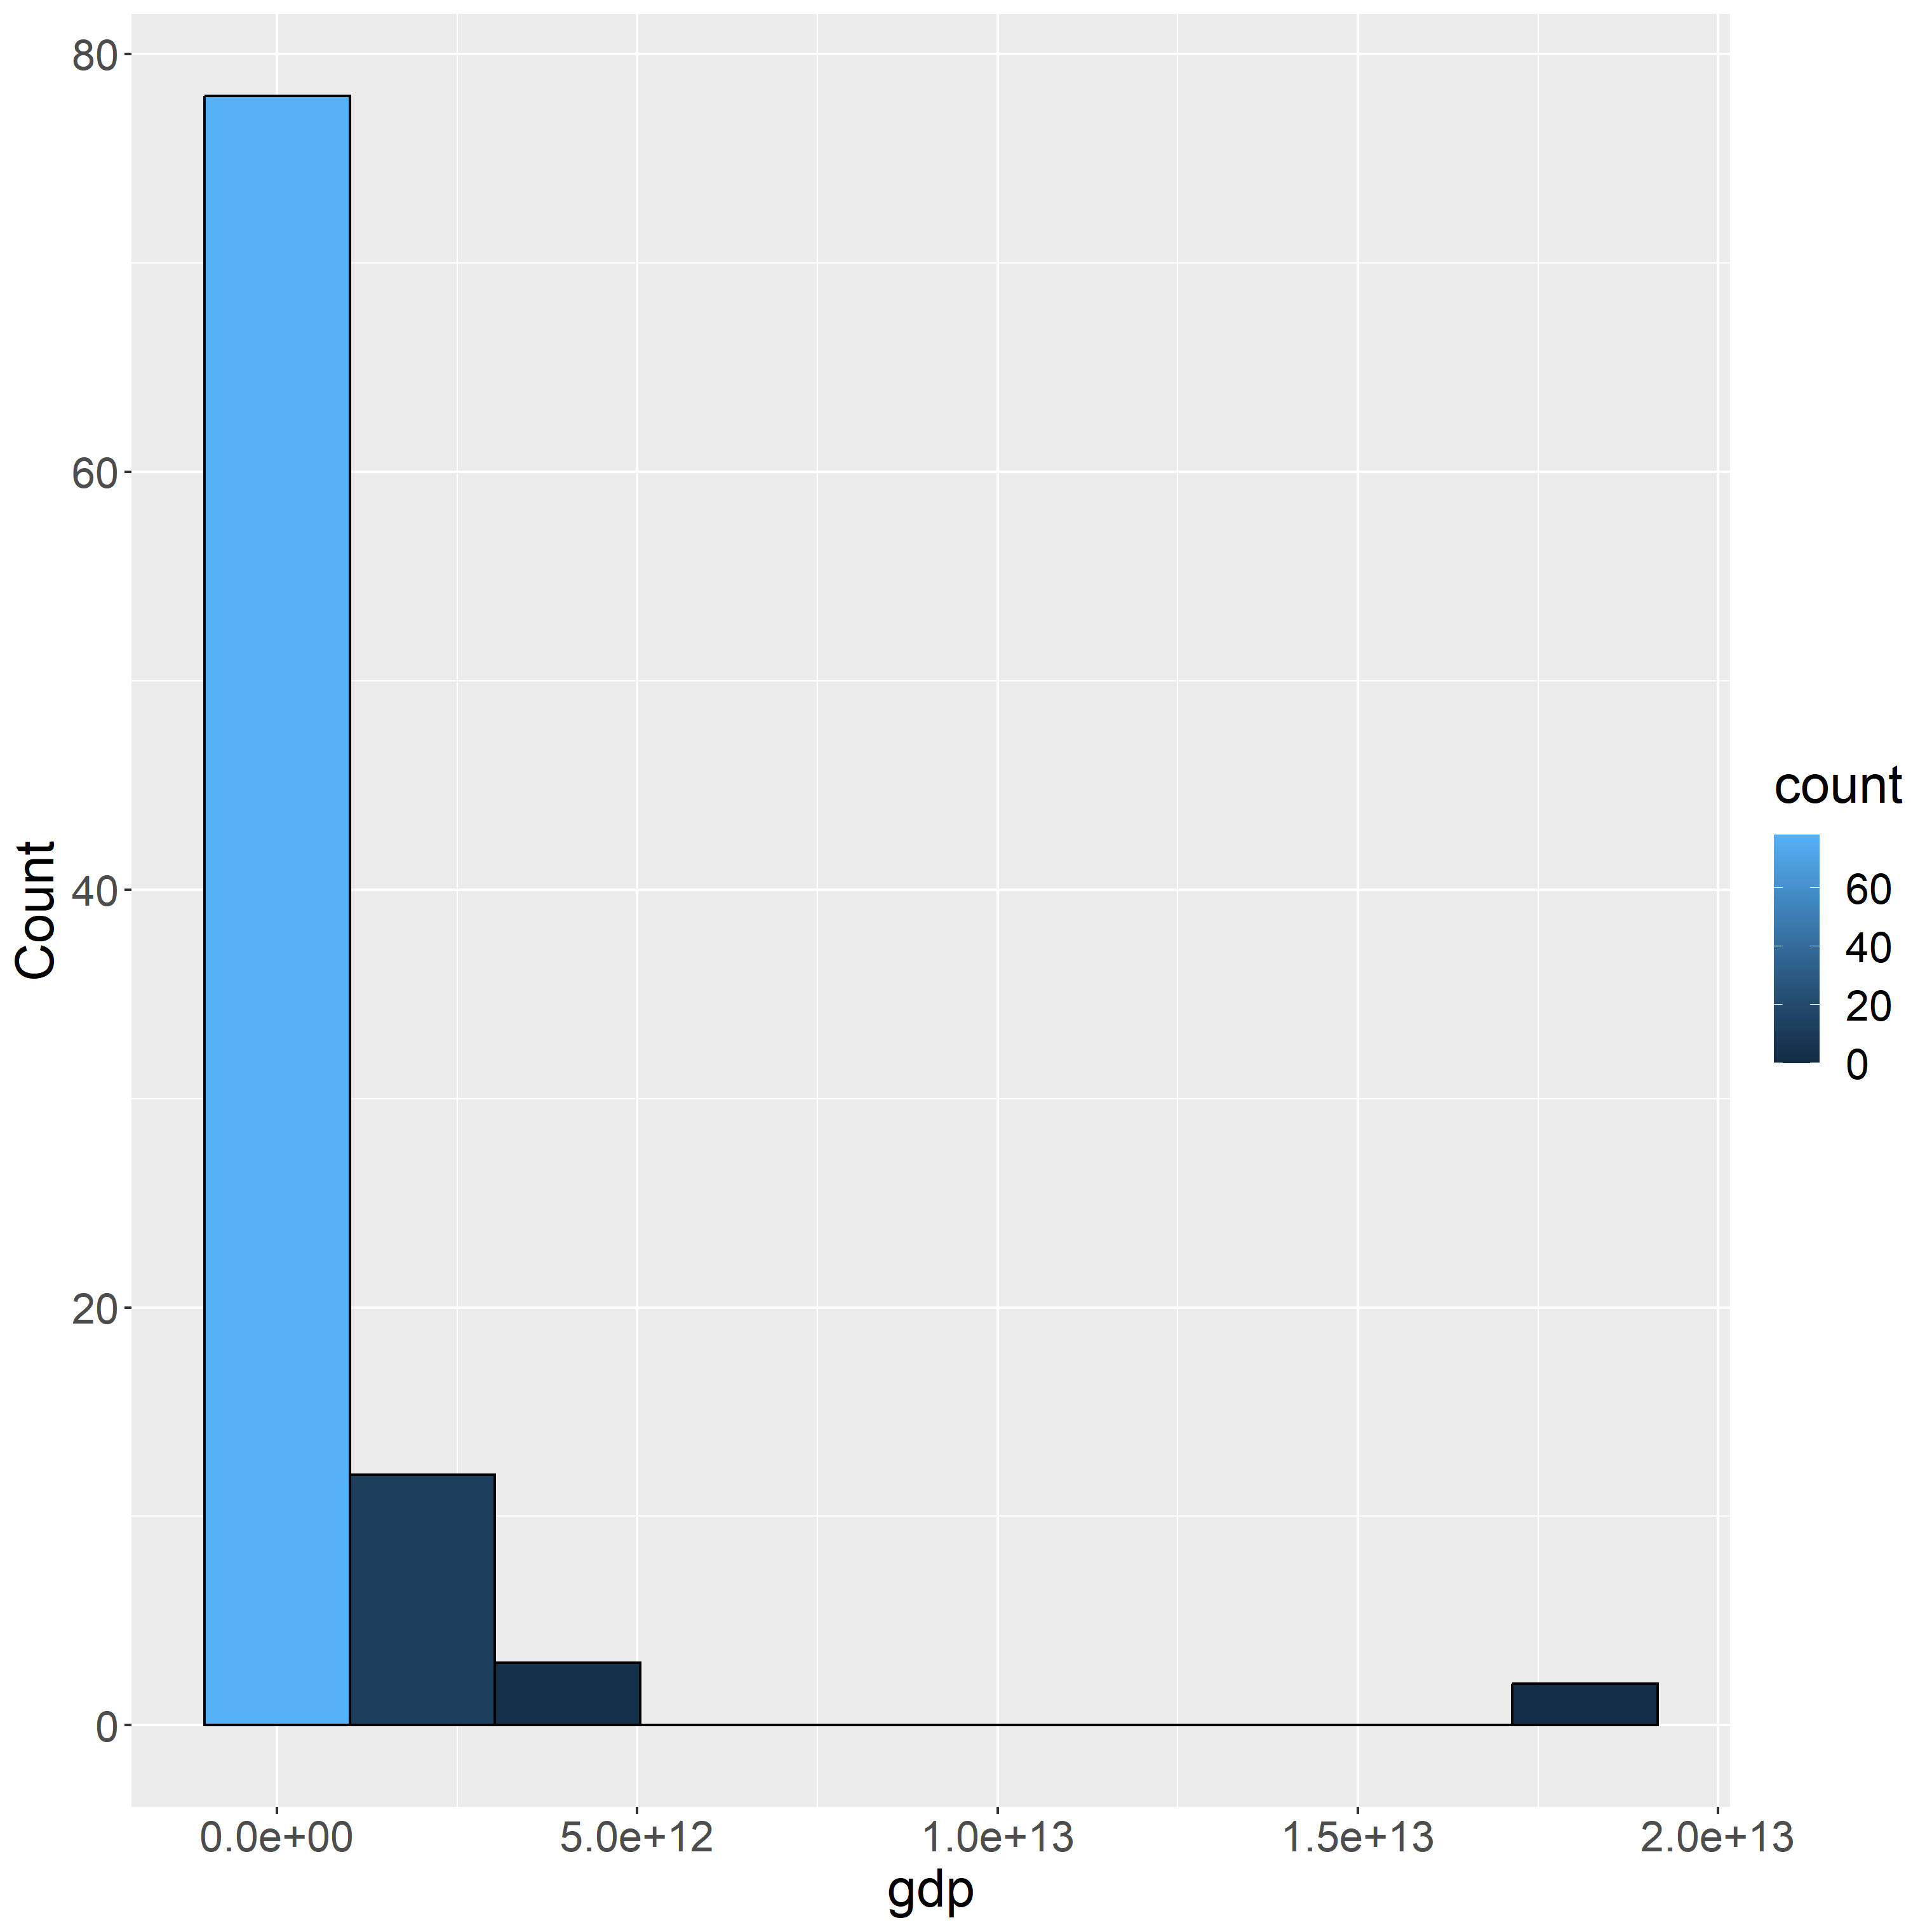
\includegraphics[width=.32\textwidth]{distribution_gdp.png}\hfill
		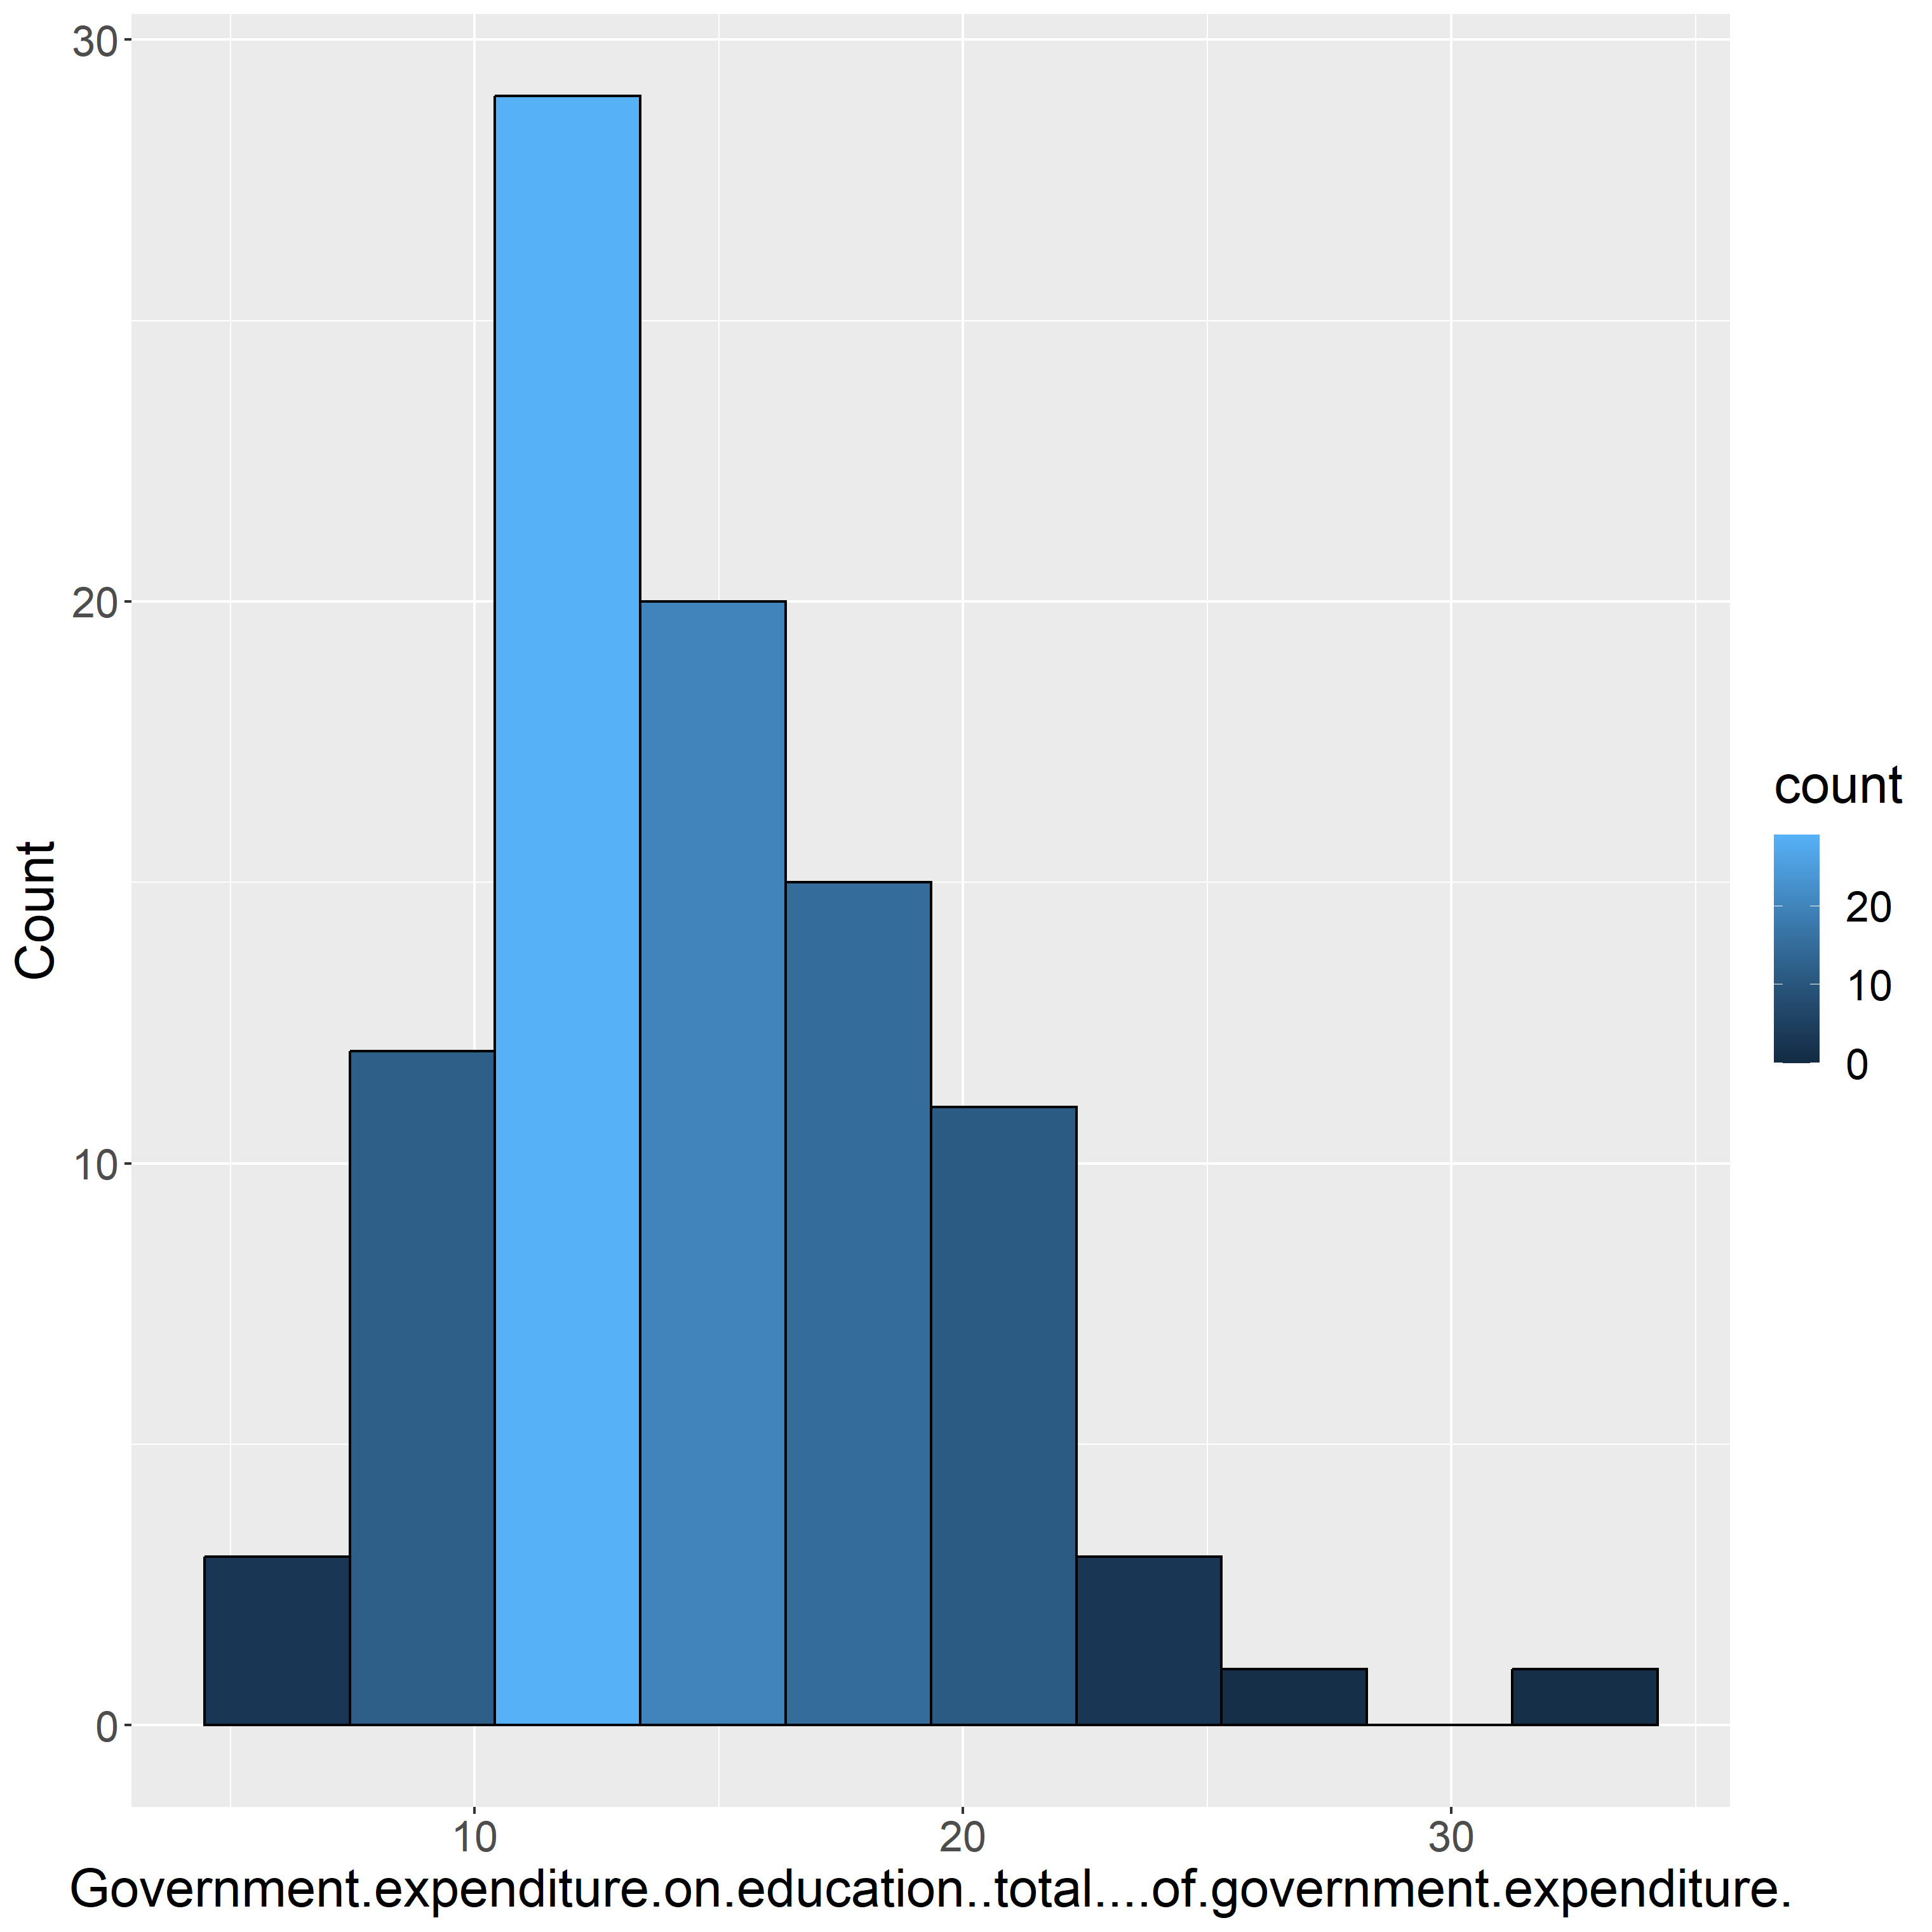
\includegraphics[width=.32\textwidth]{distribution_Government expenditure on education, total ( of government expenditure).png}\hfill
		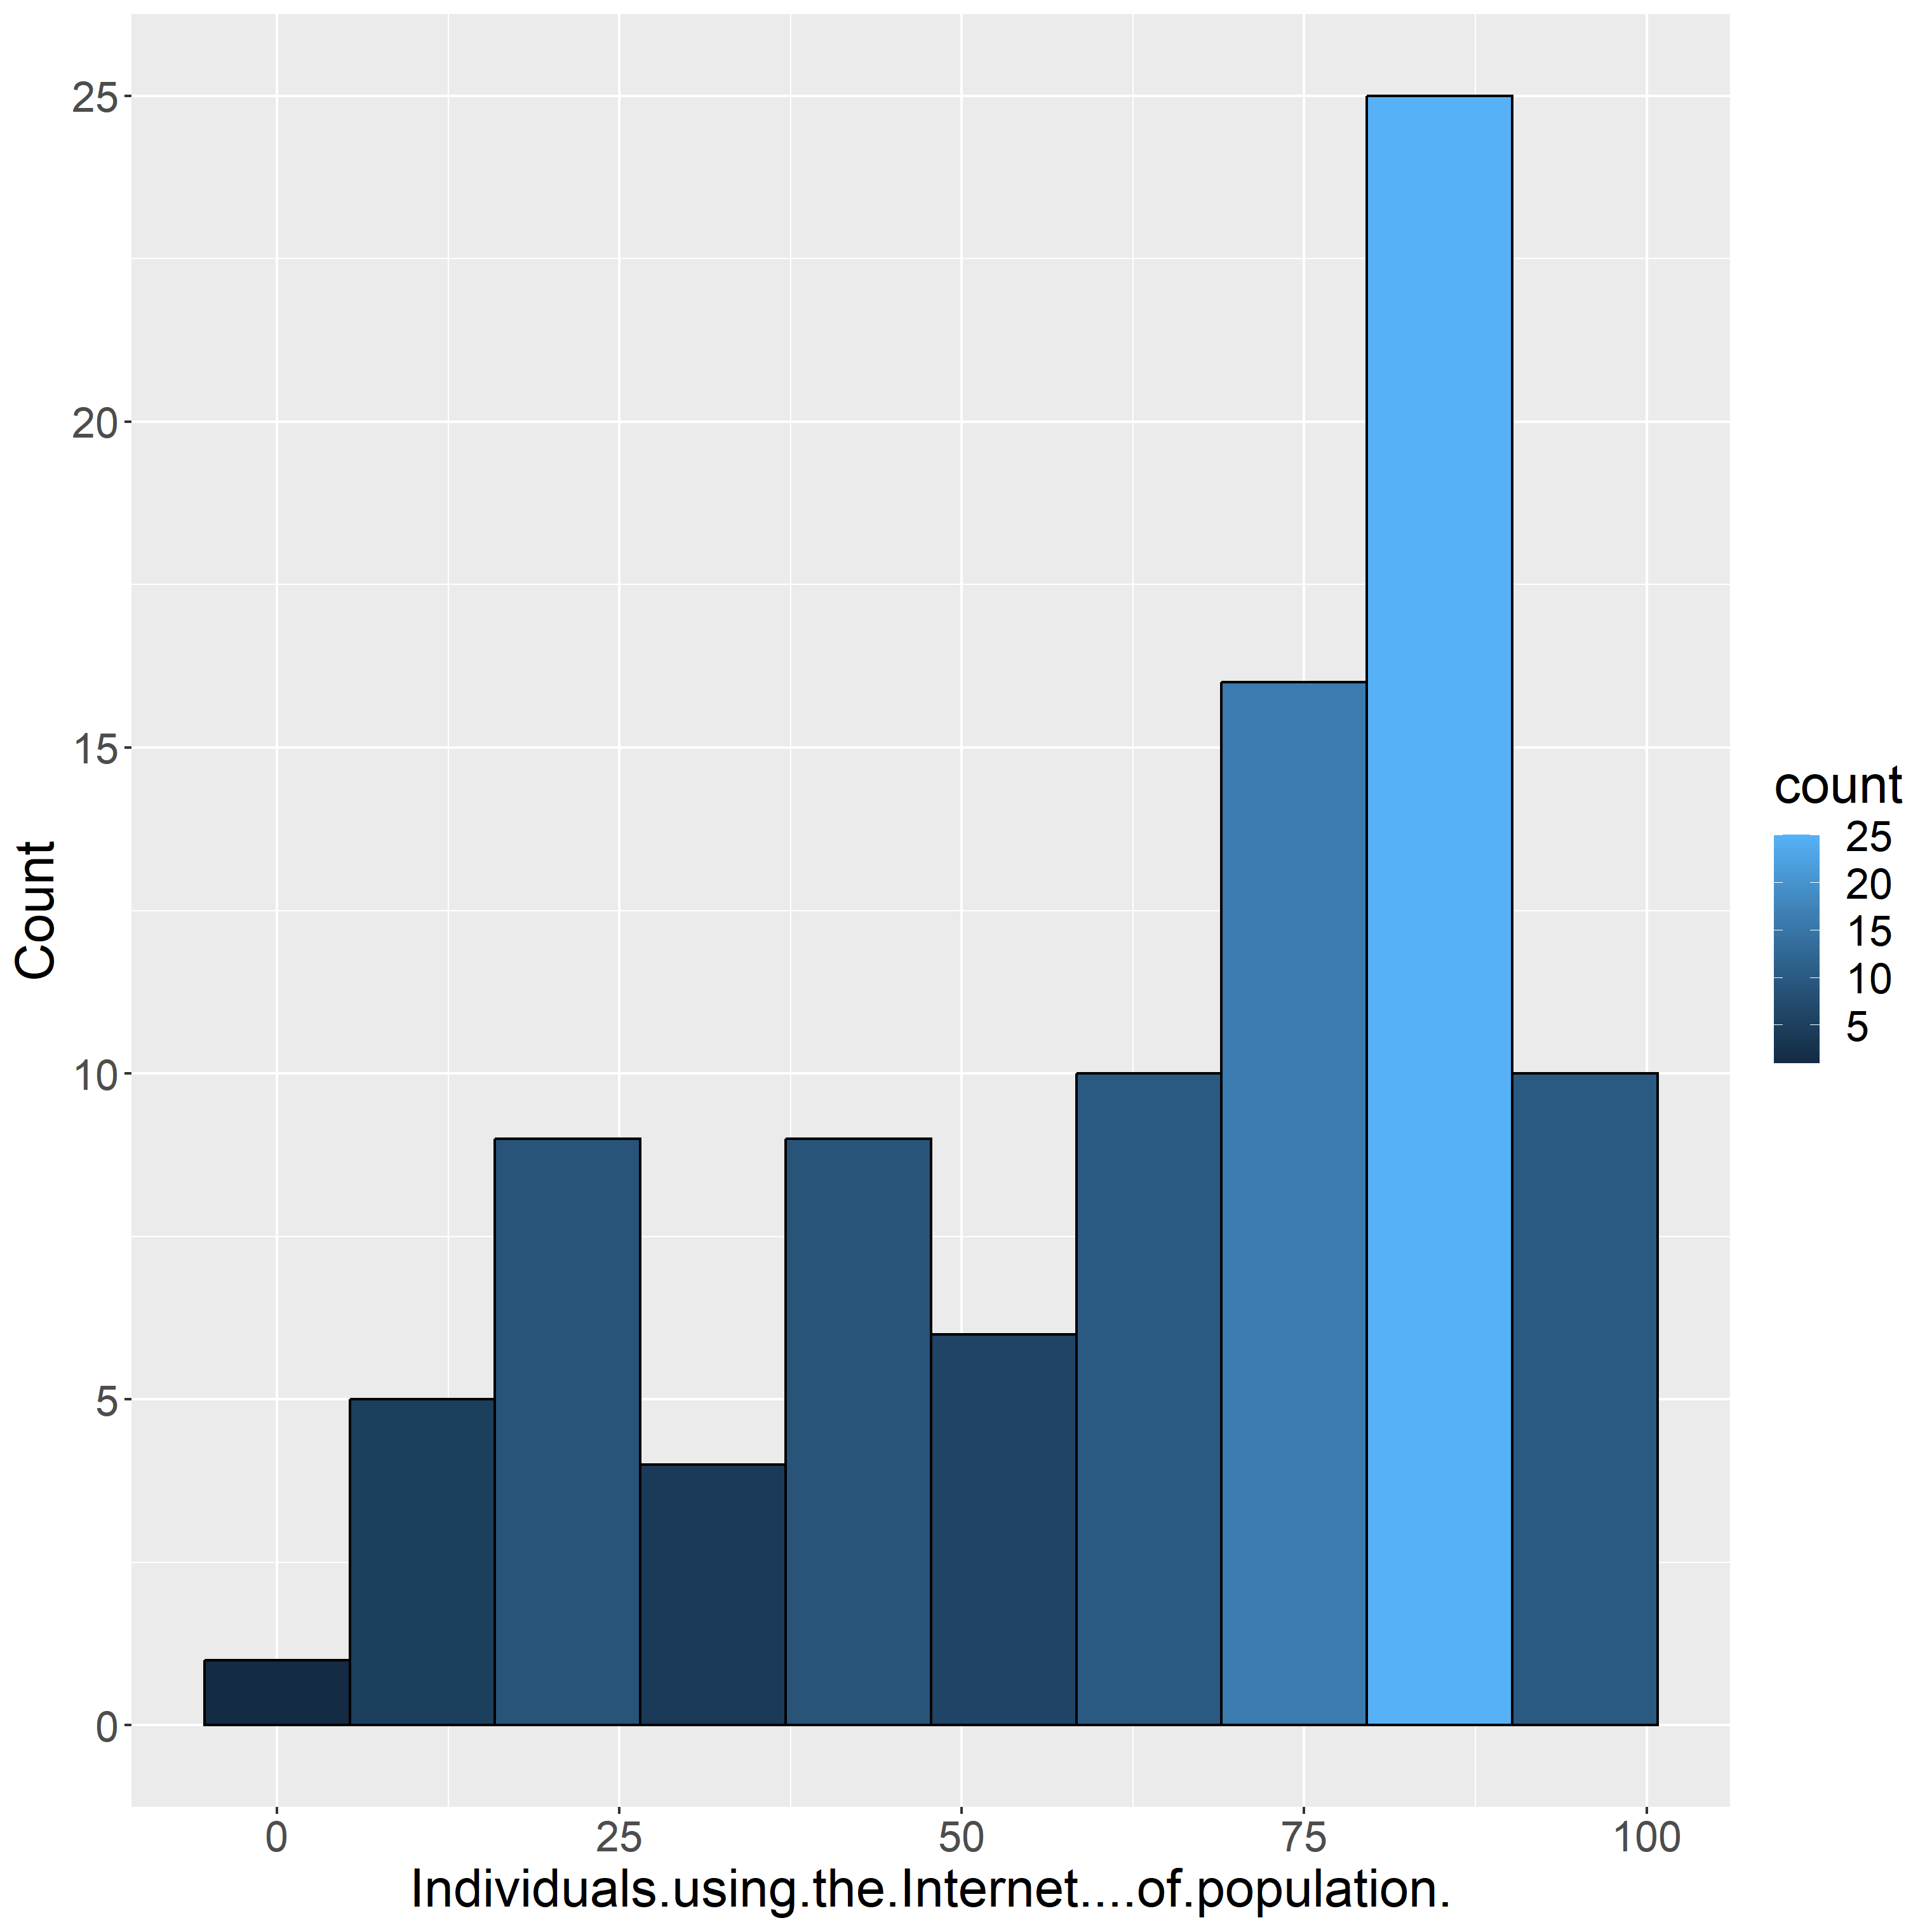
\includegraphics[width=.32\textwidth]{distribution_Individuals using the Internet ( of population).png}
		\\[\smallskipamount]
		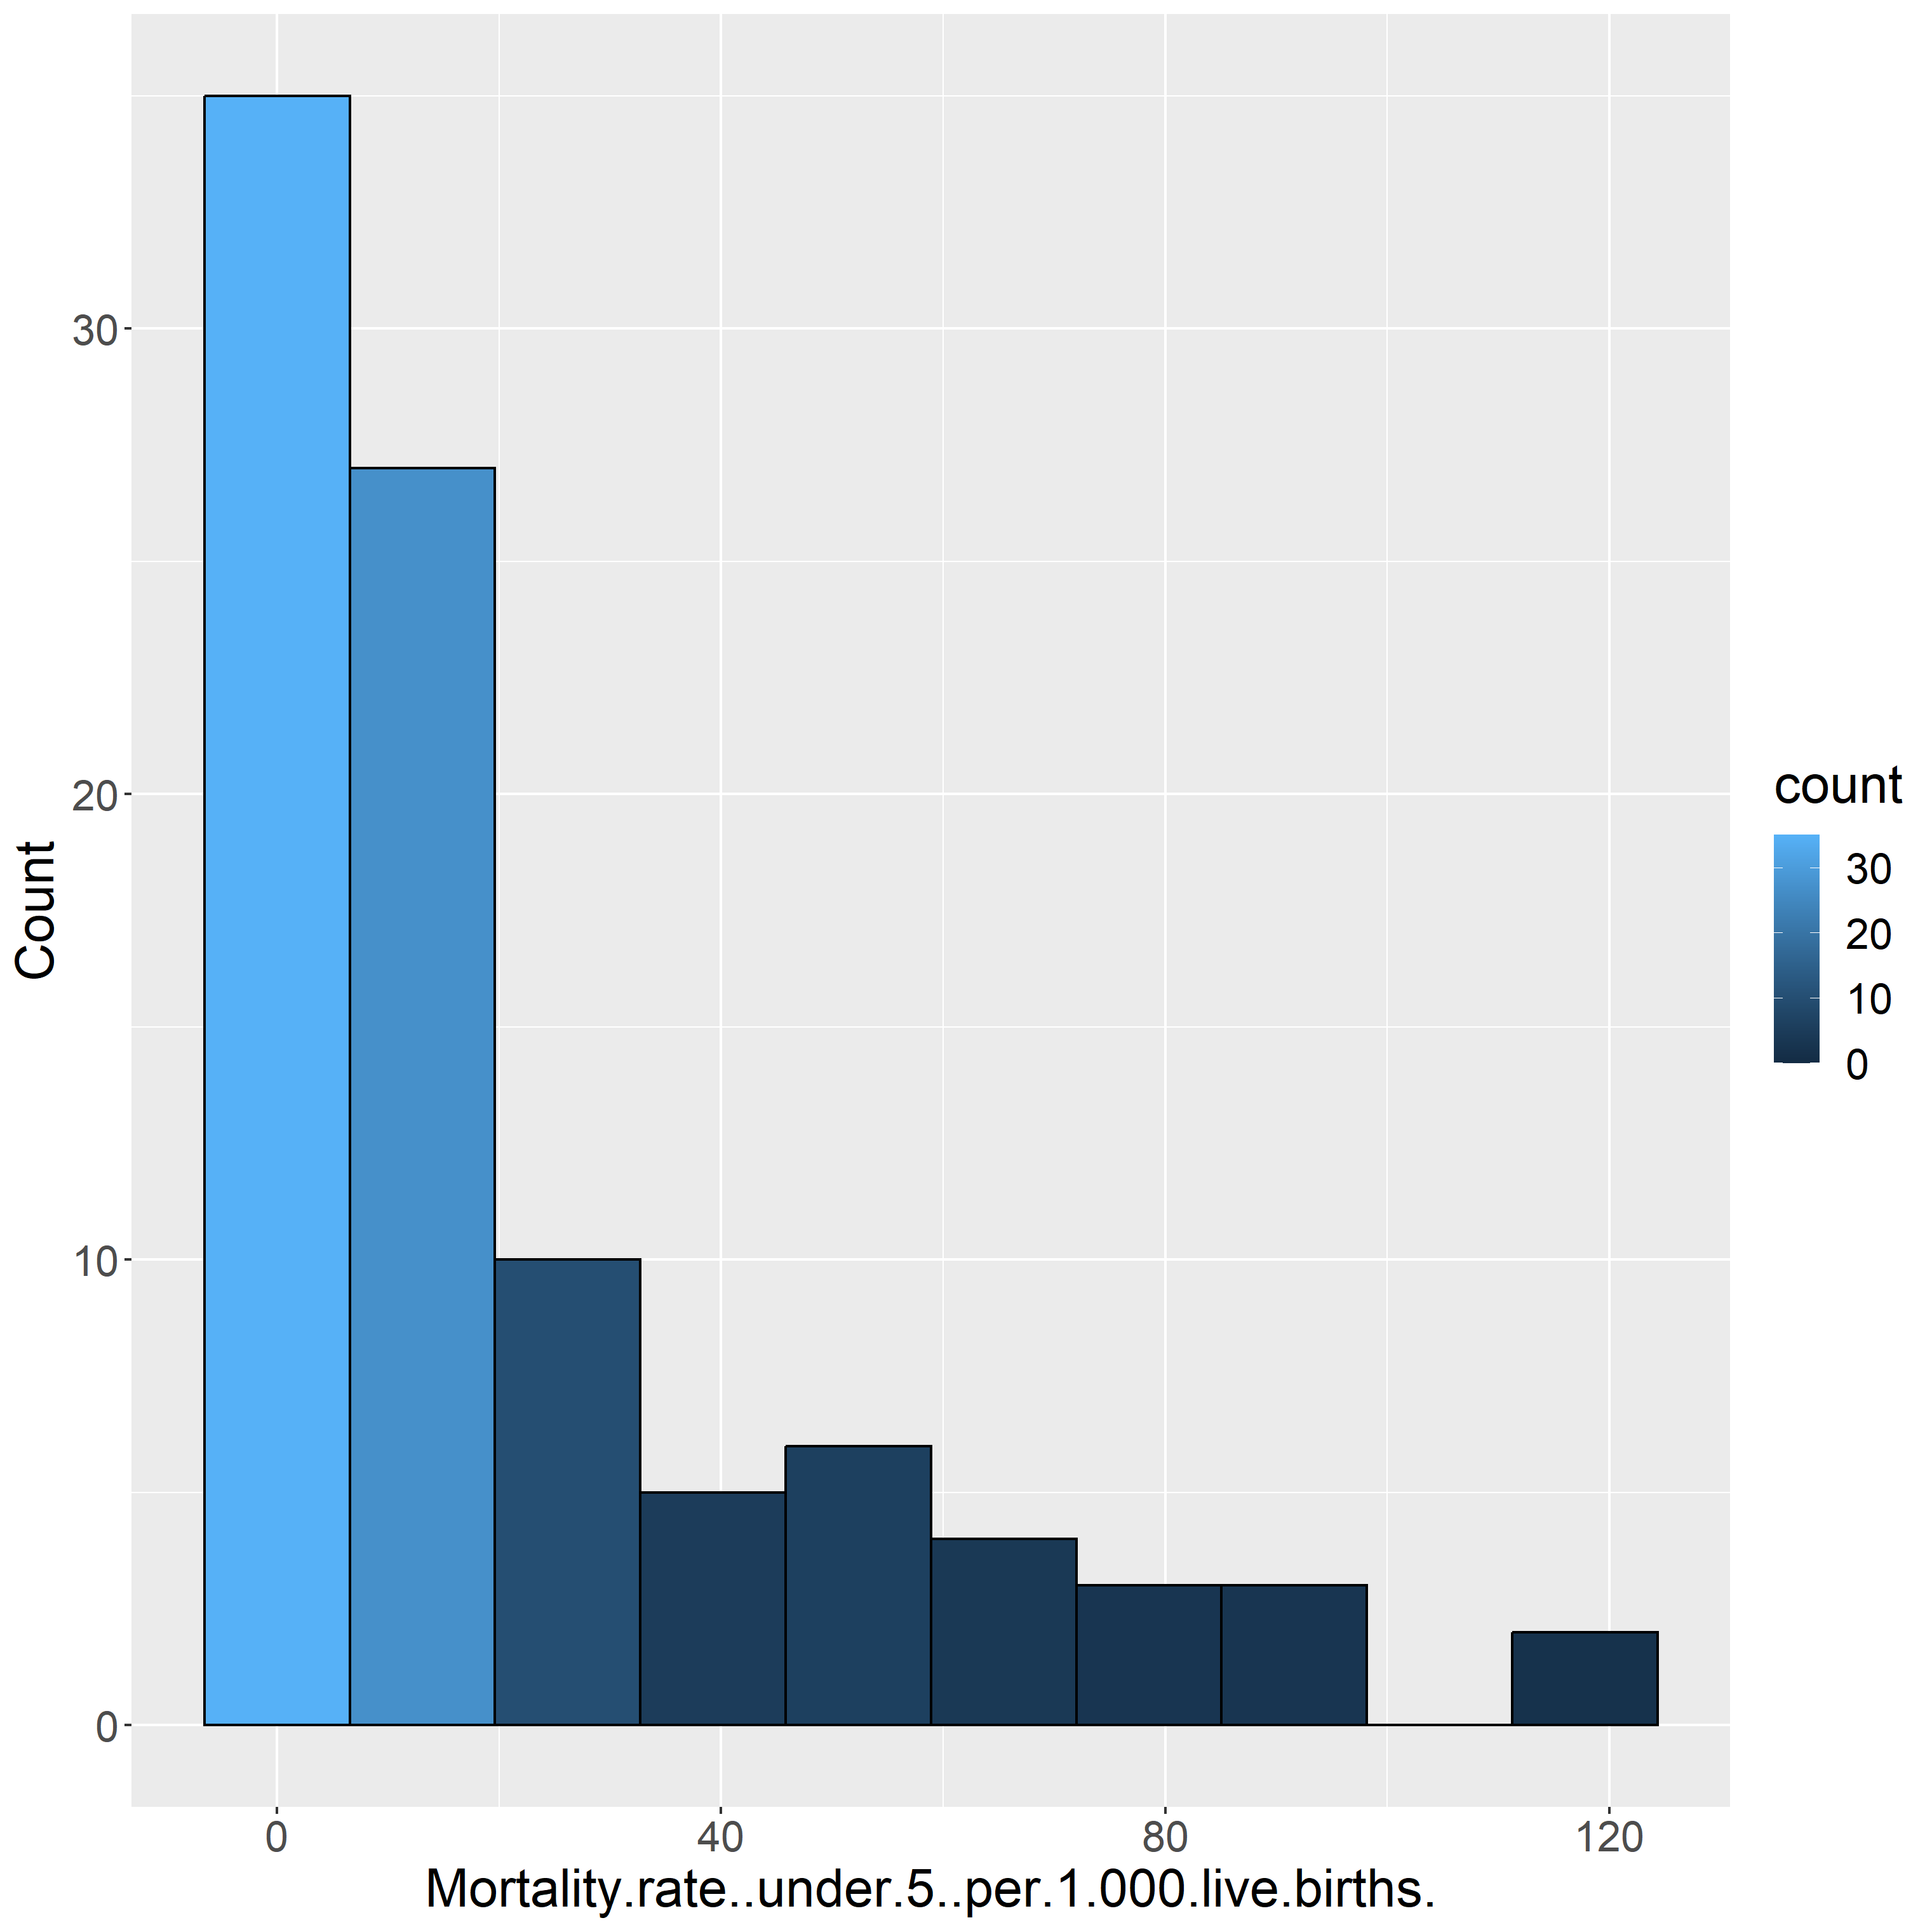
\includegraphics[width=.32\textwidth]{distribution_Mortality rate, under-5 (per 1,000 live births).png}\hfill
		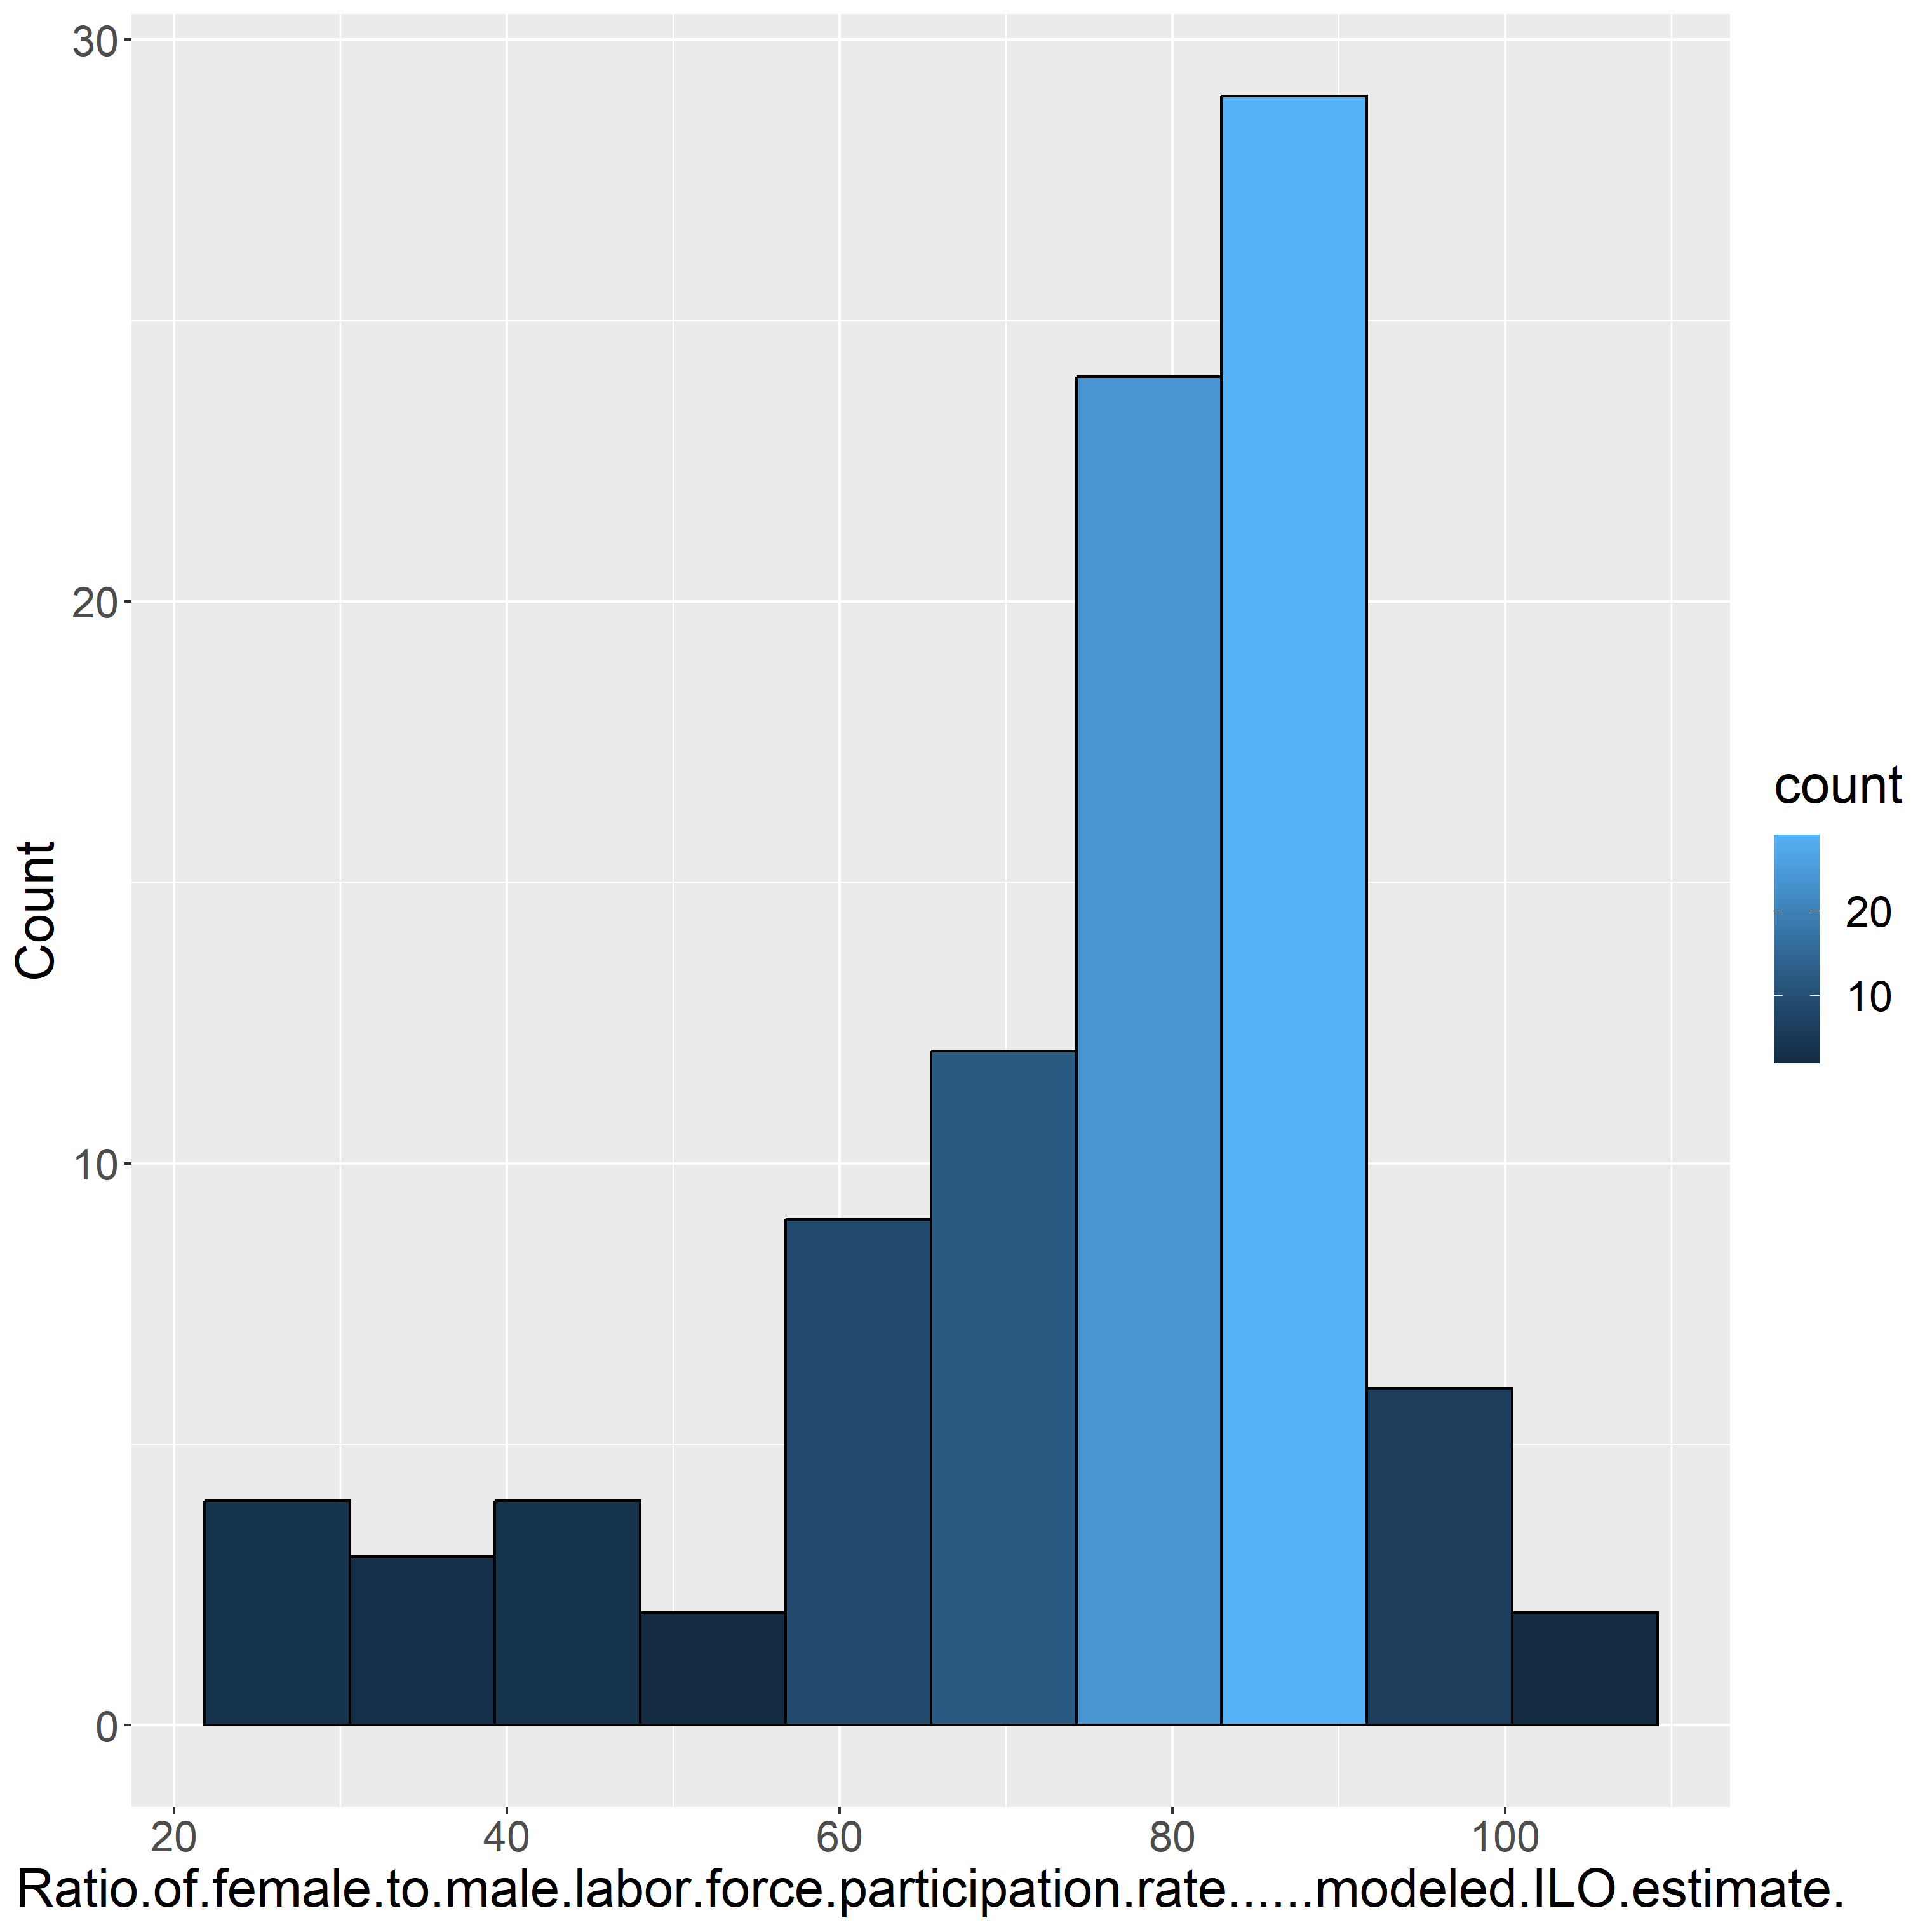
\includegraphics[width=.32\textwidth]{distribution_Ratio of female to male labor force participation rate () (modeled ILO estimate).png}\hfill
		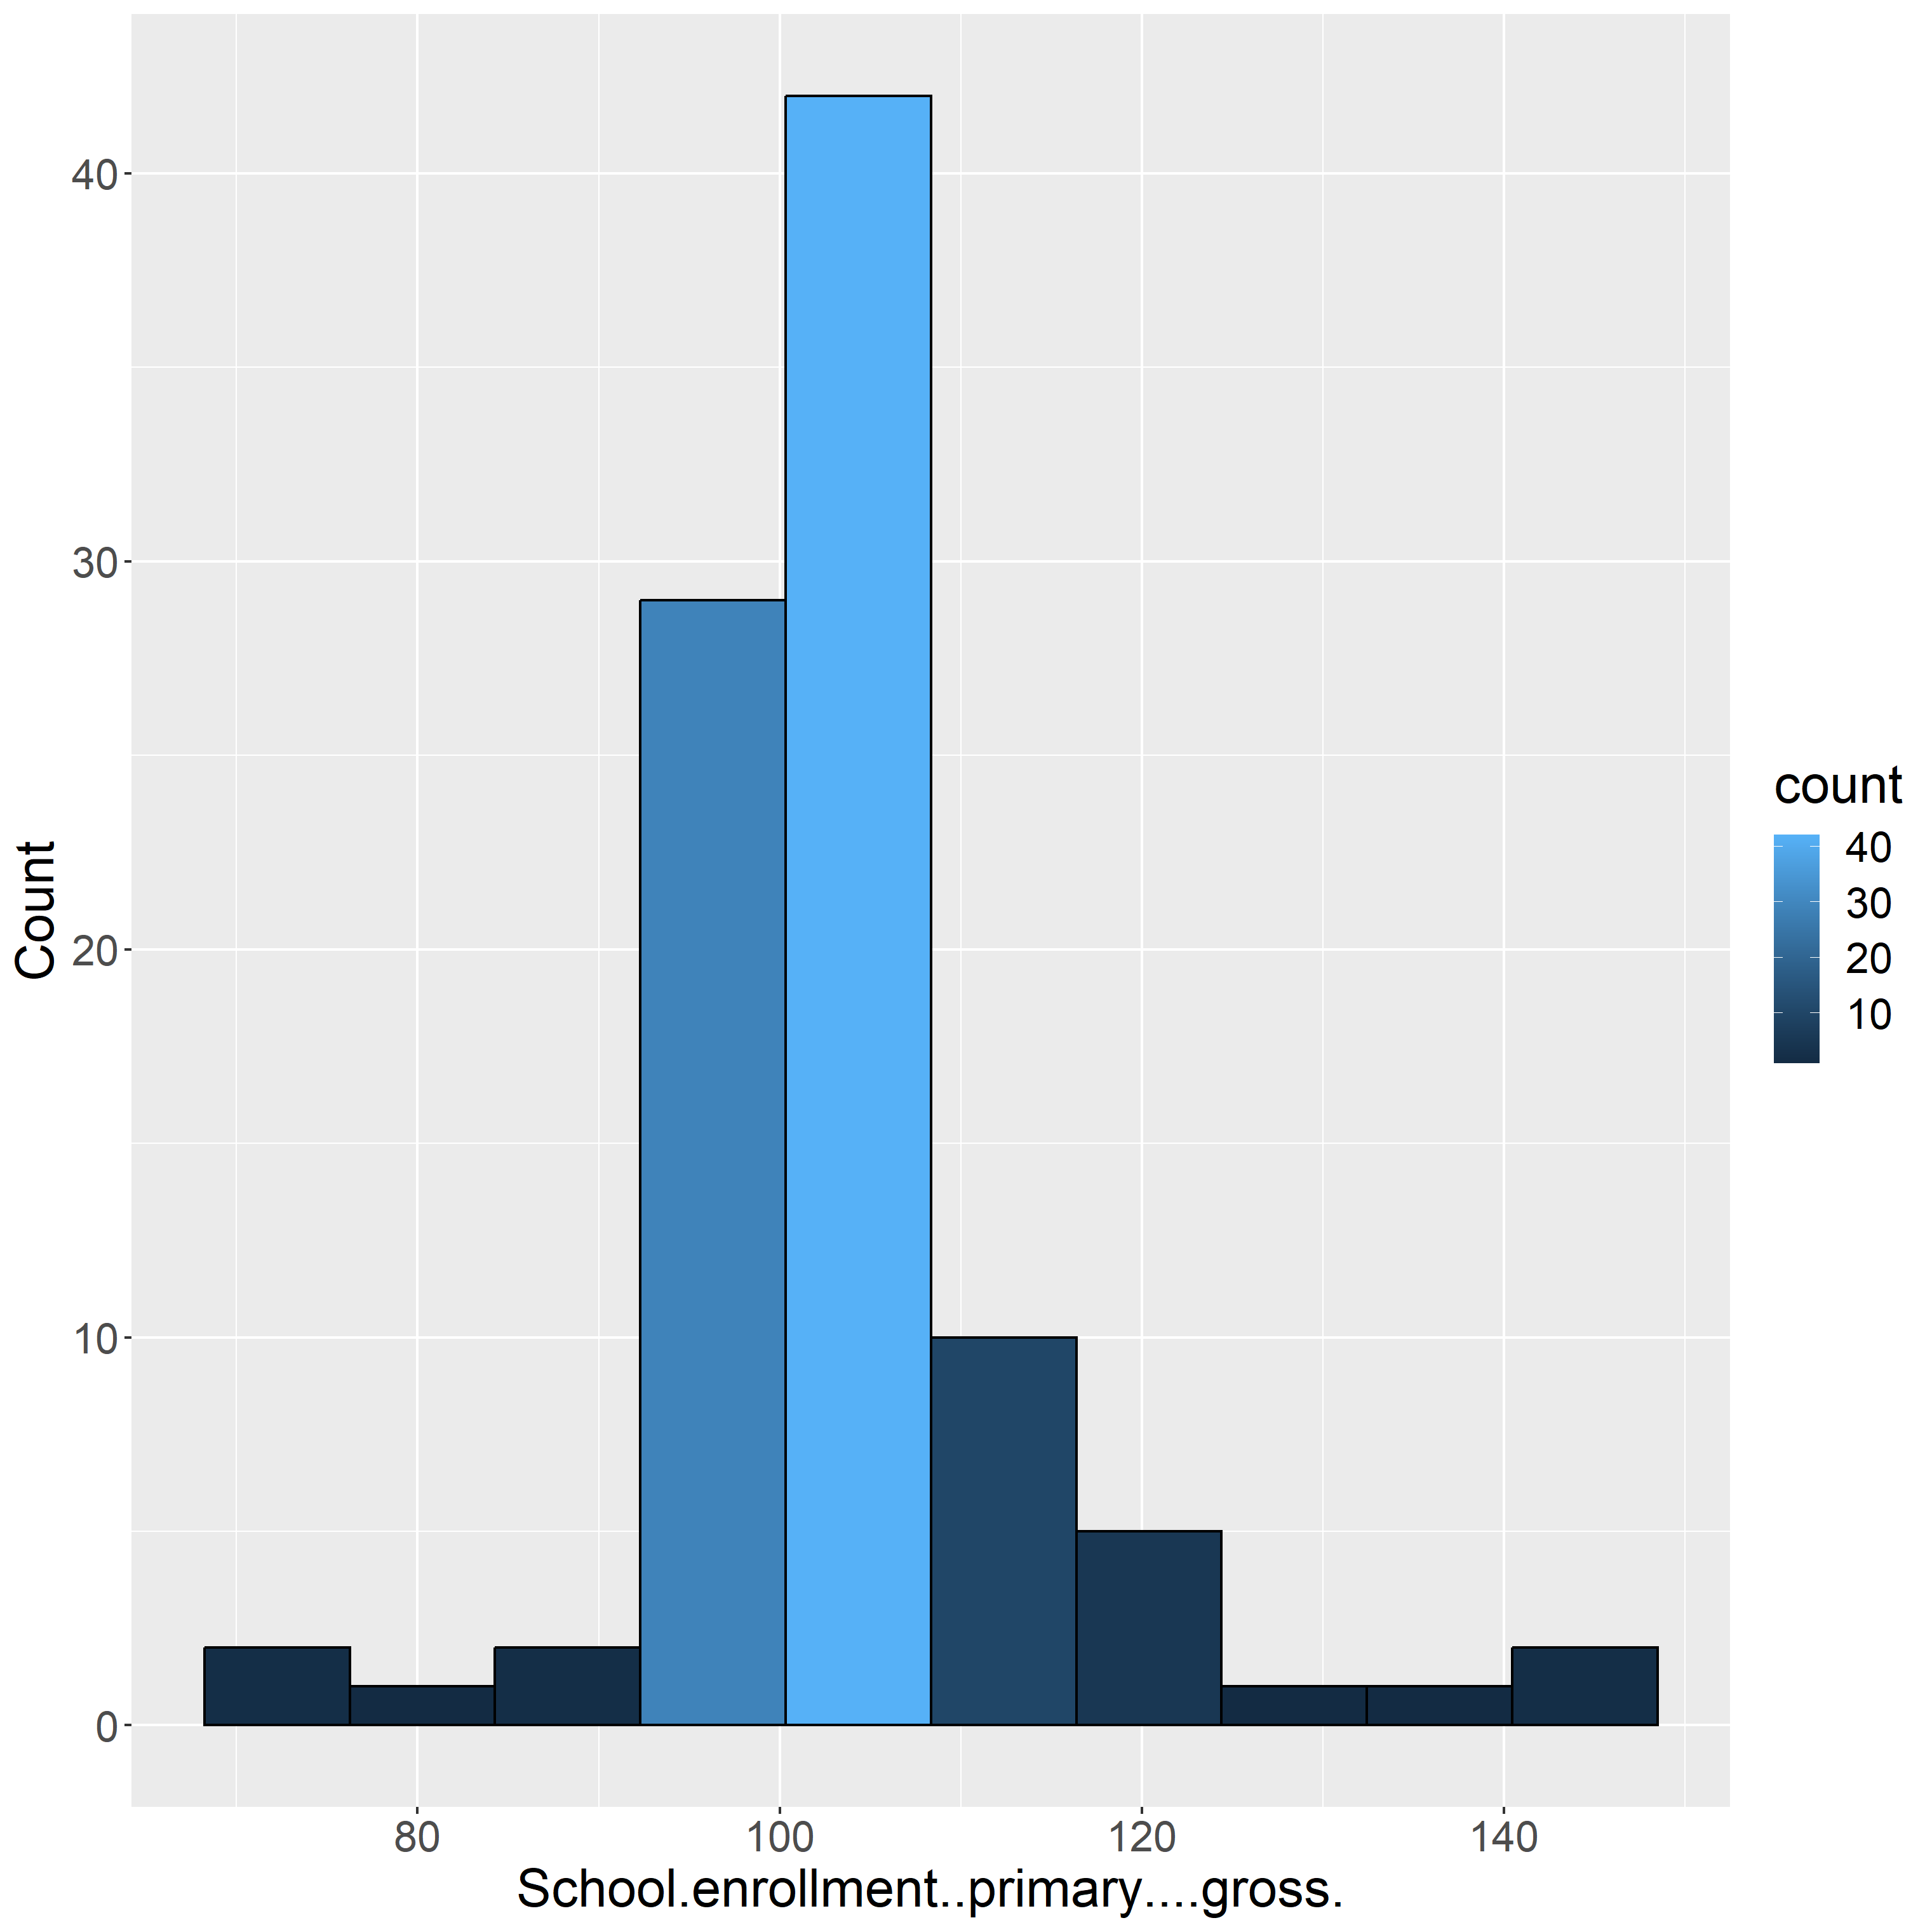
\includegraphics[width=.32\textwidth]{distribution_School enrollment, primary ( gross).png}\hfill
		\\[\smallskipamount]
		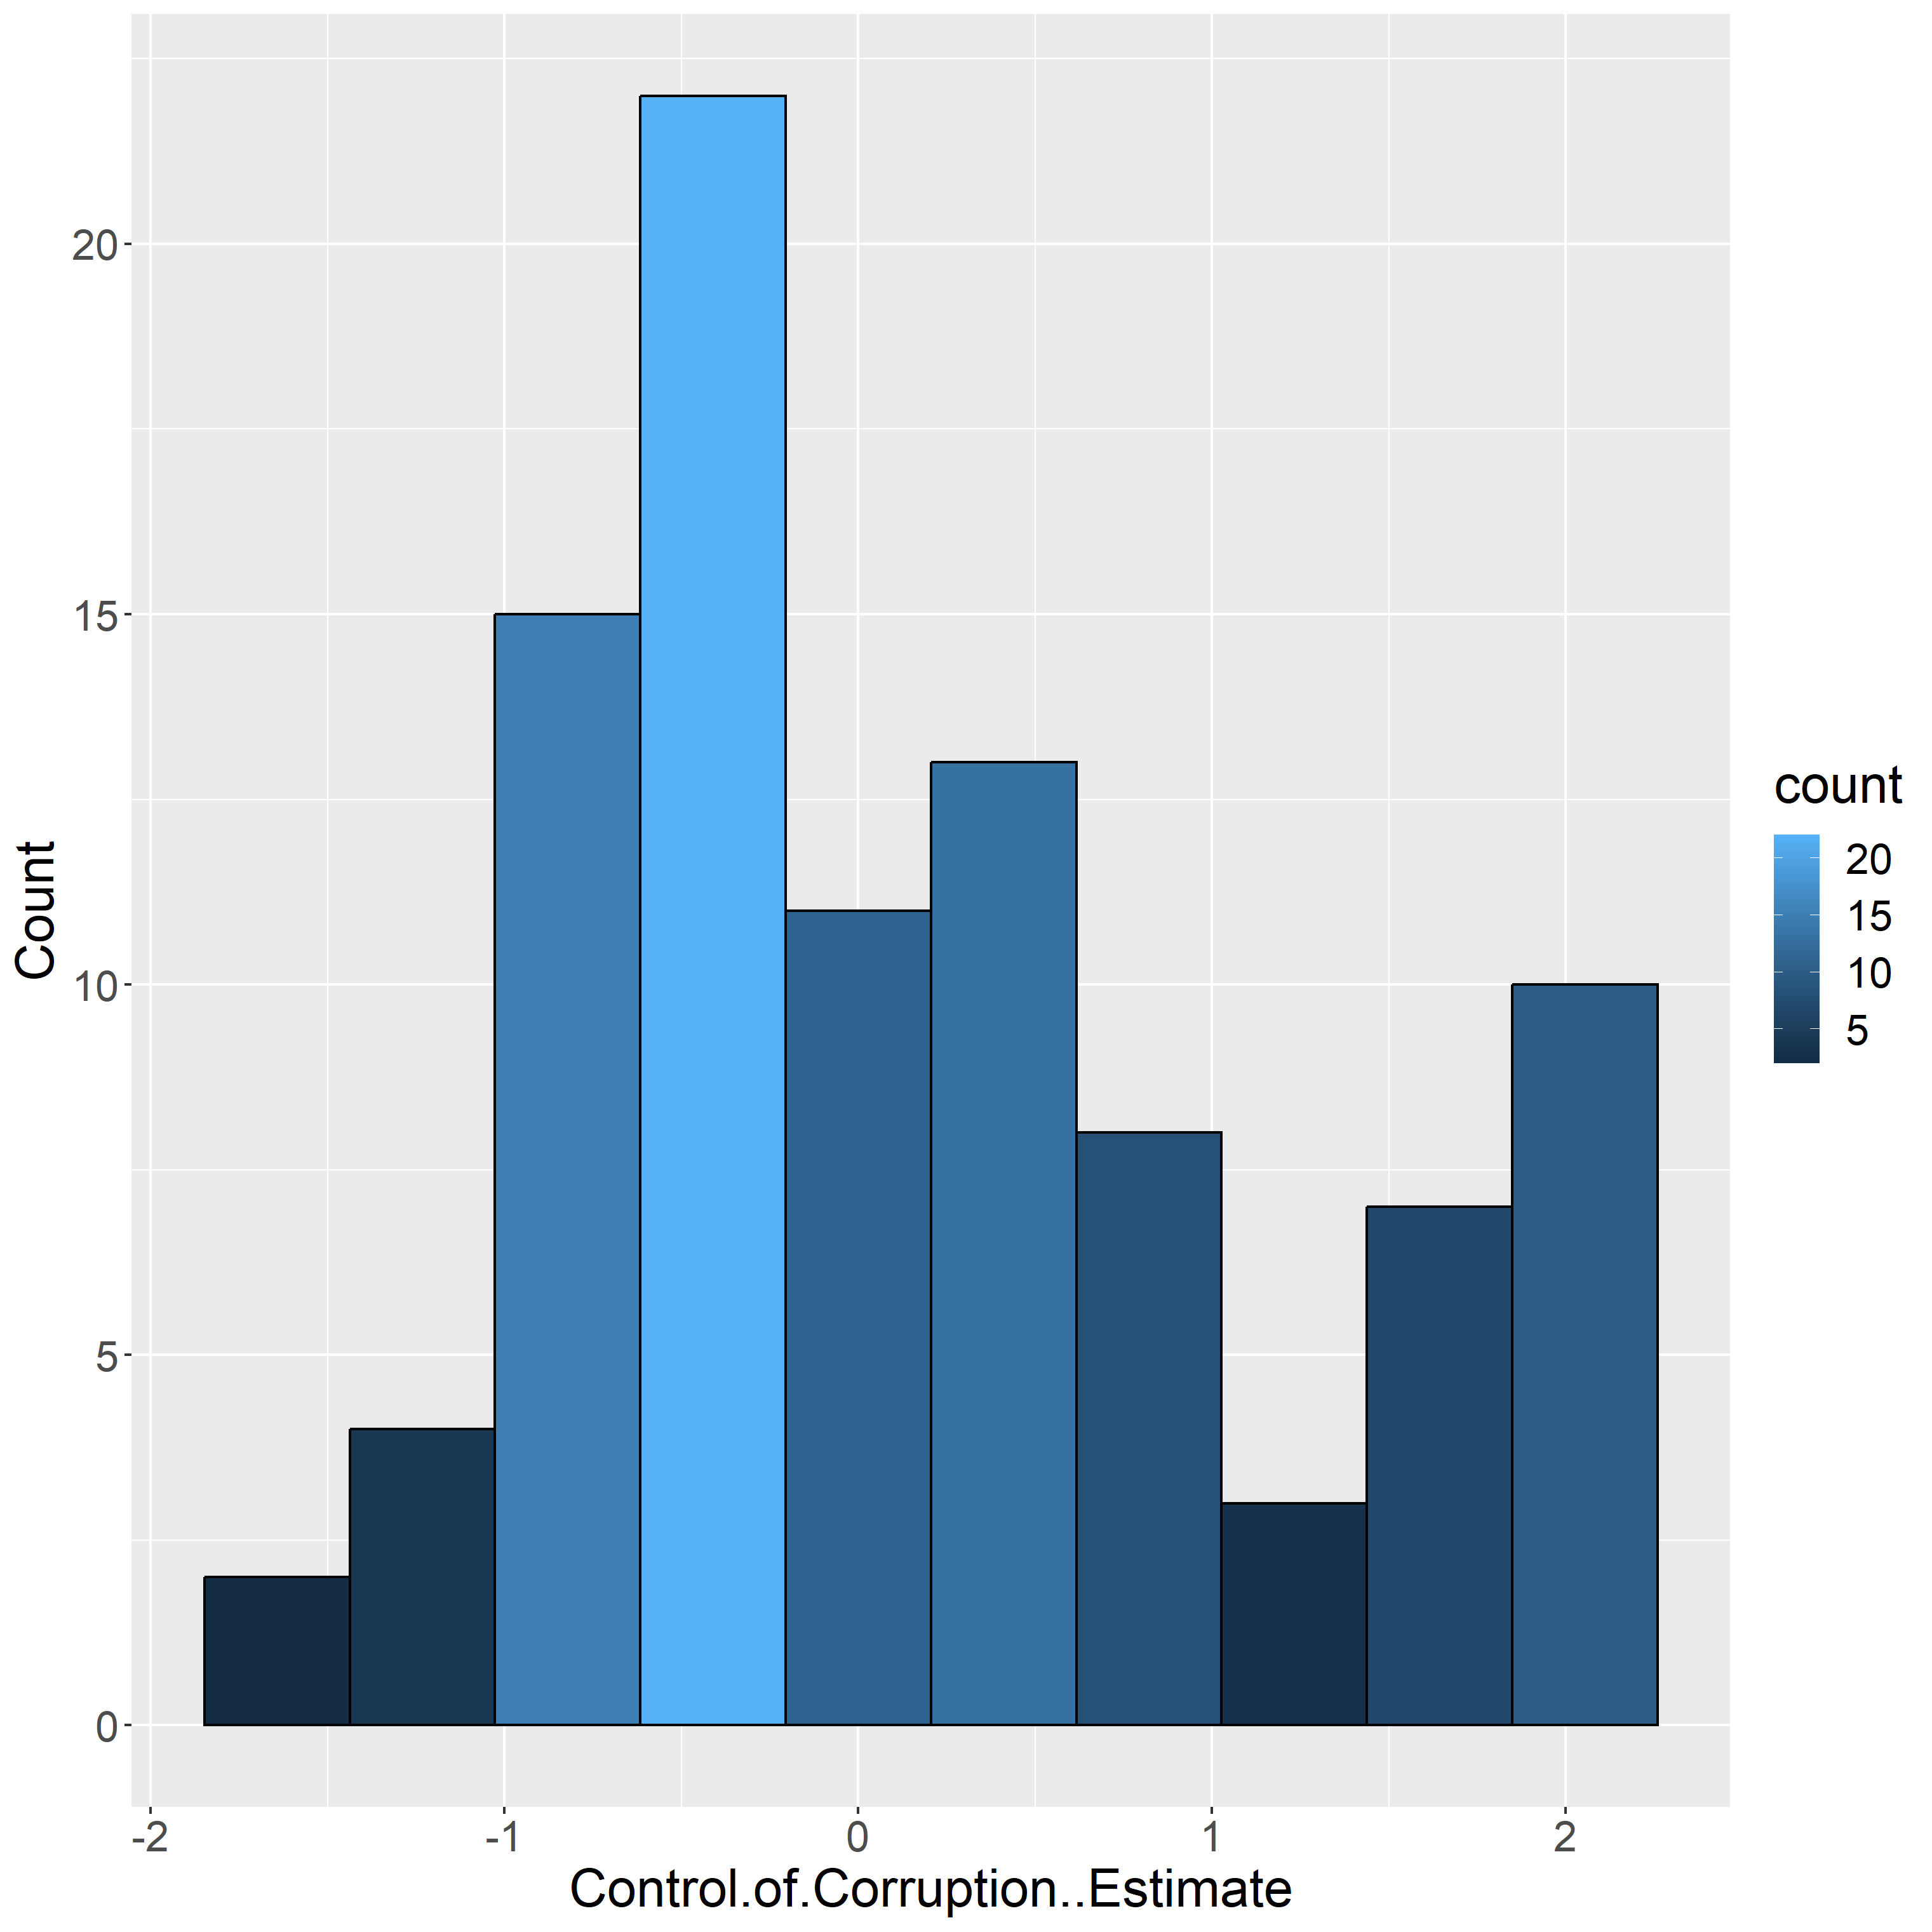
\includegraphics[width=.32\textwidth]{distribution_Control of Corruption- Estimate.png}
		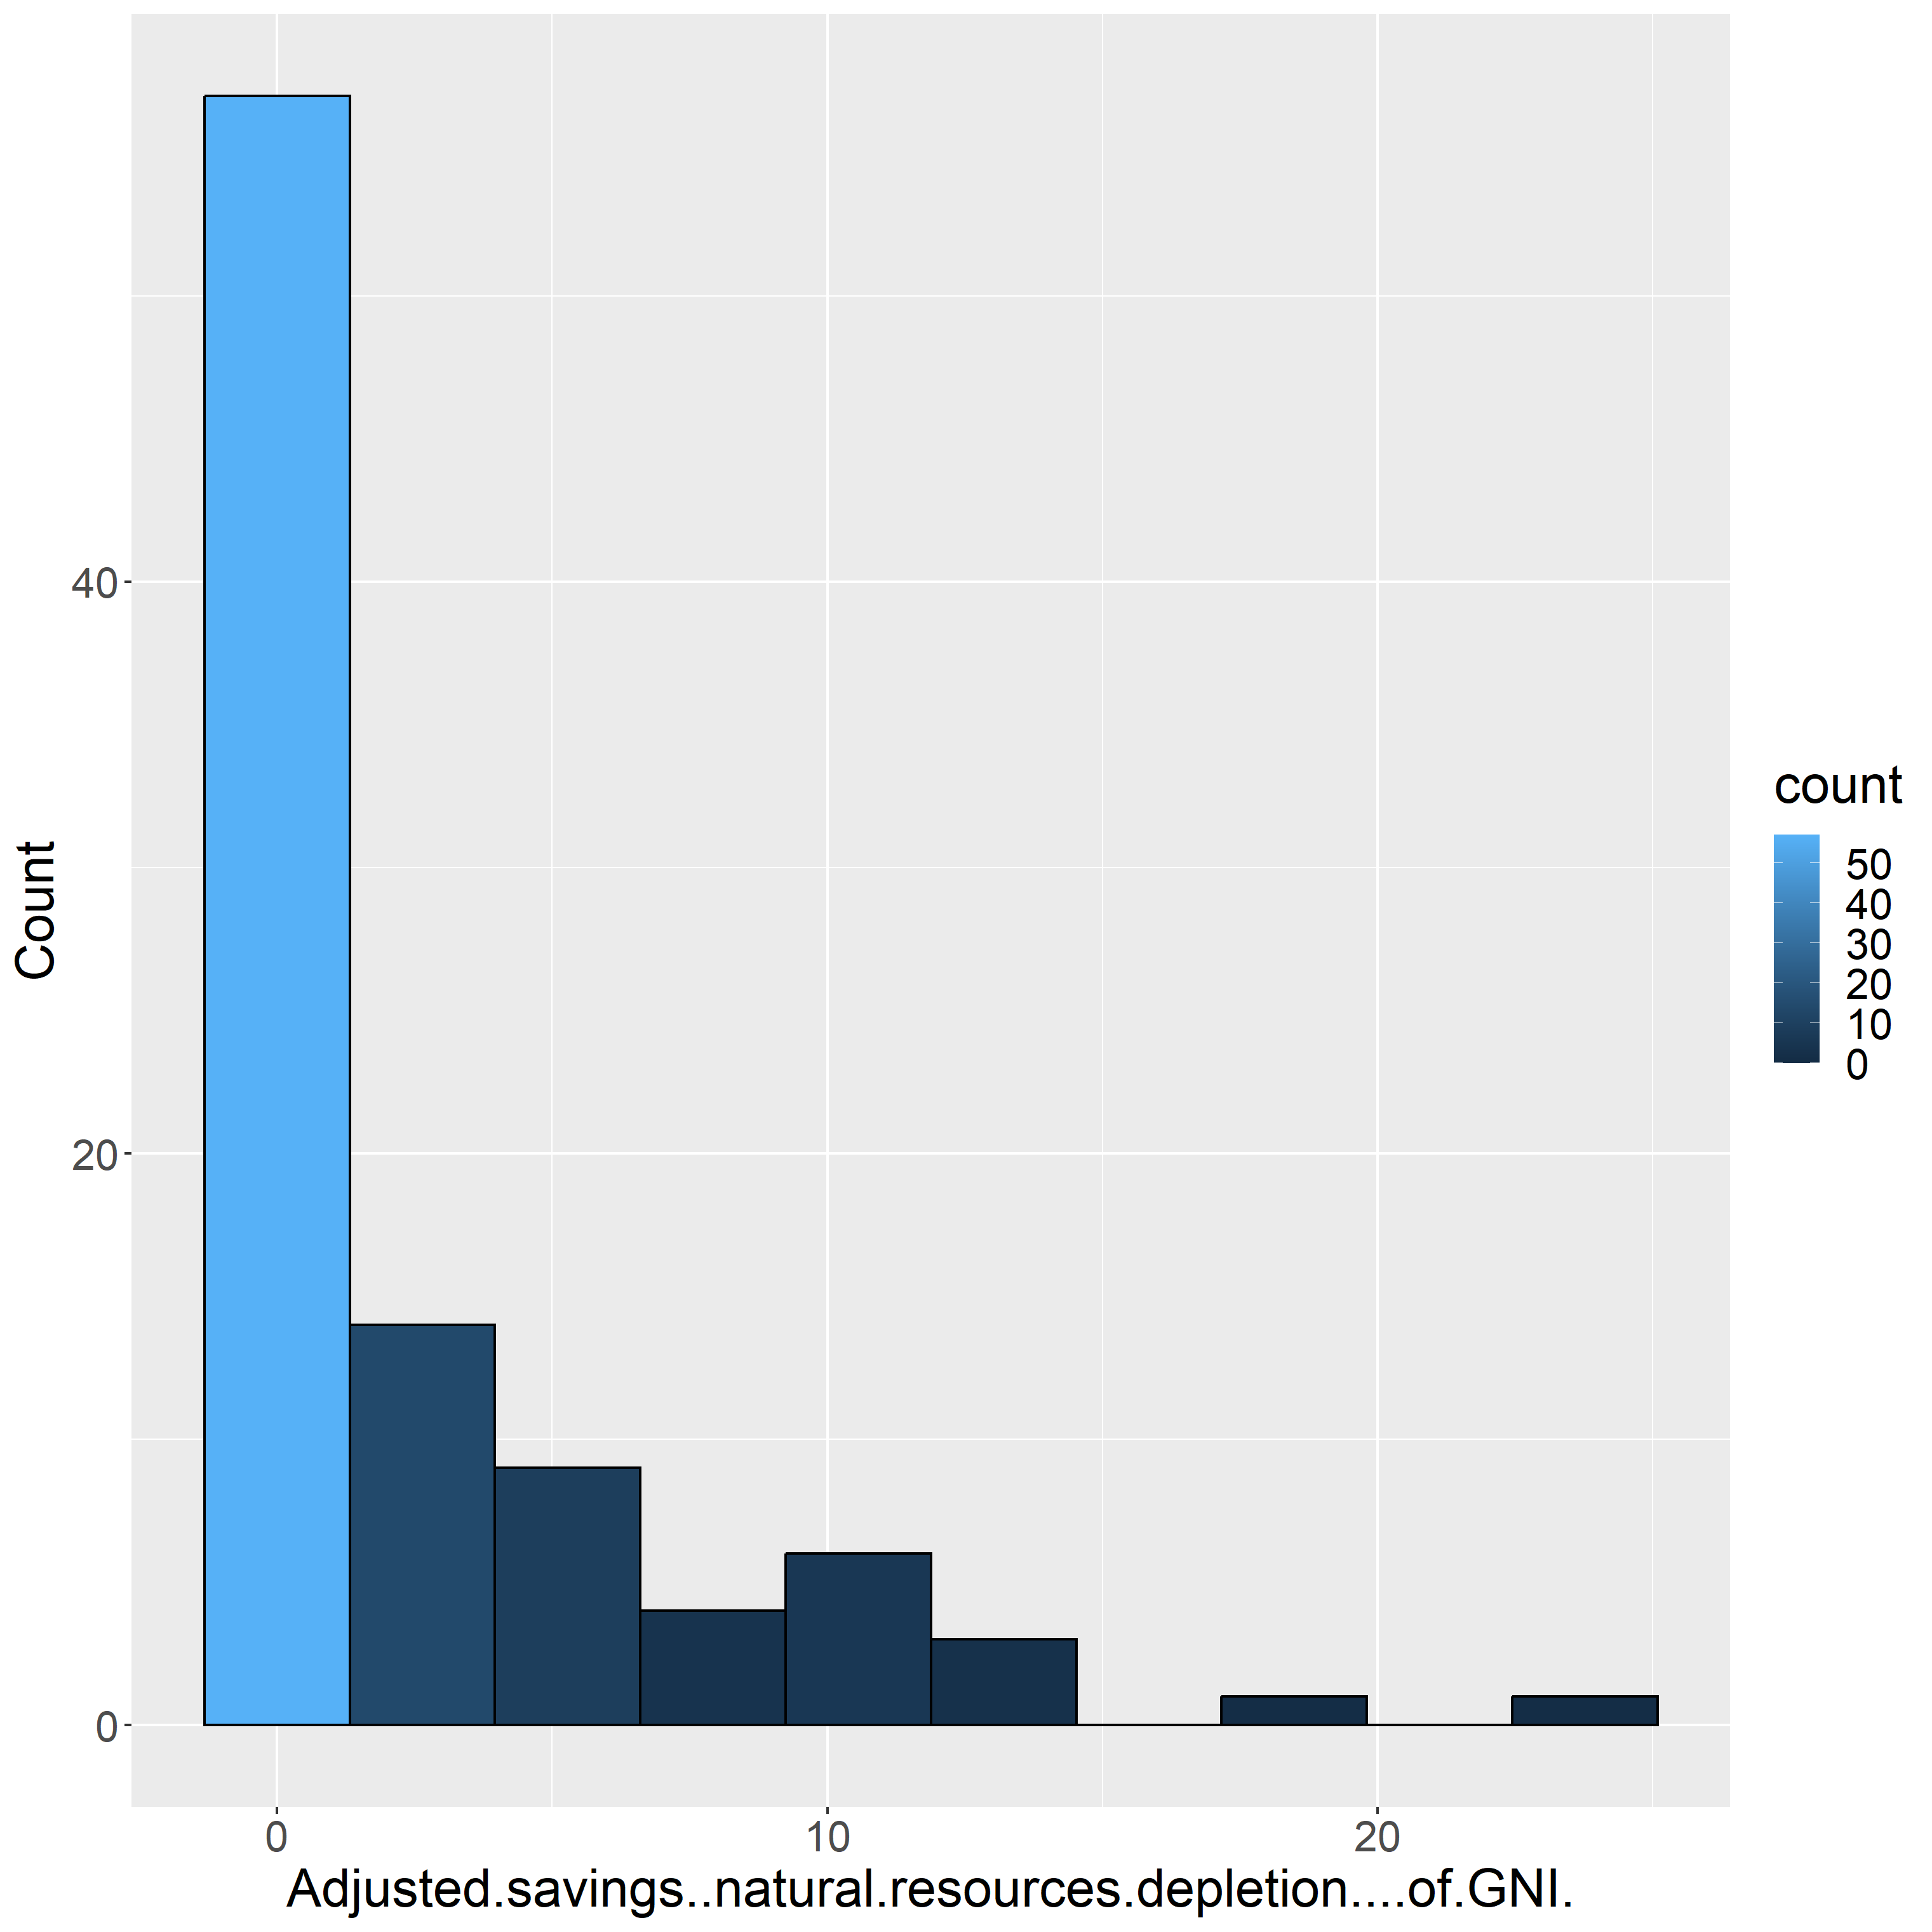
\includegraphics[width=.32\textwidth]{distribution_Adjusted savings- natural resources depletion ( of GNI).png}\hfill
		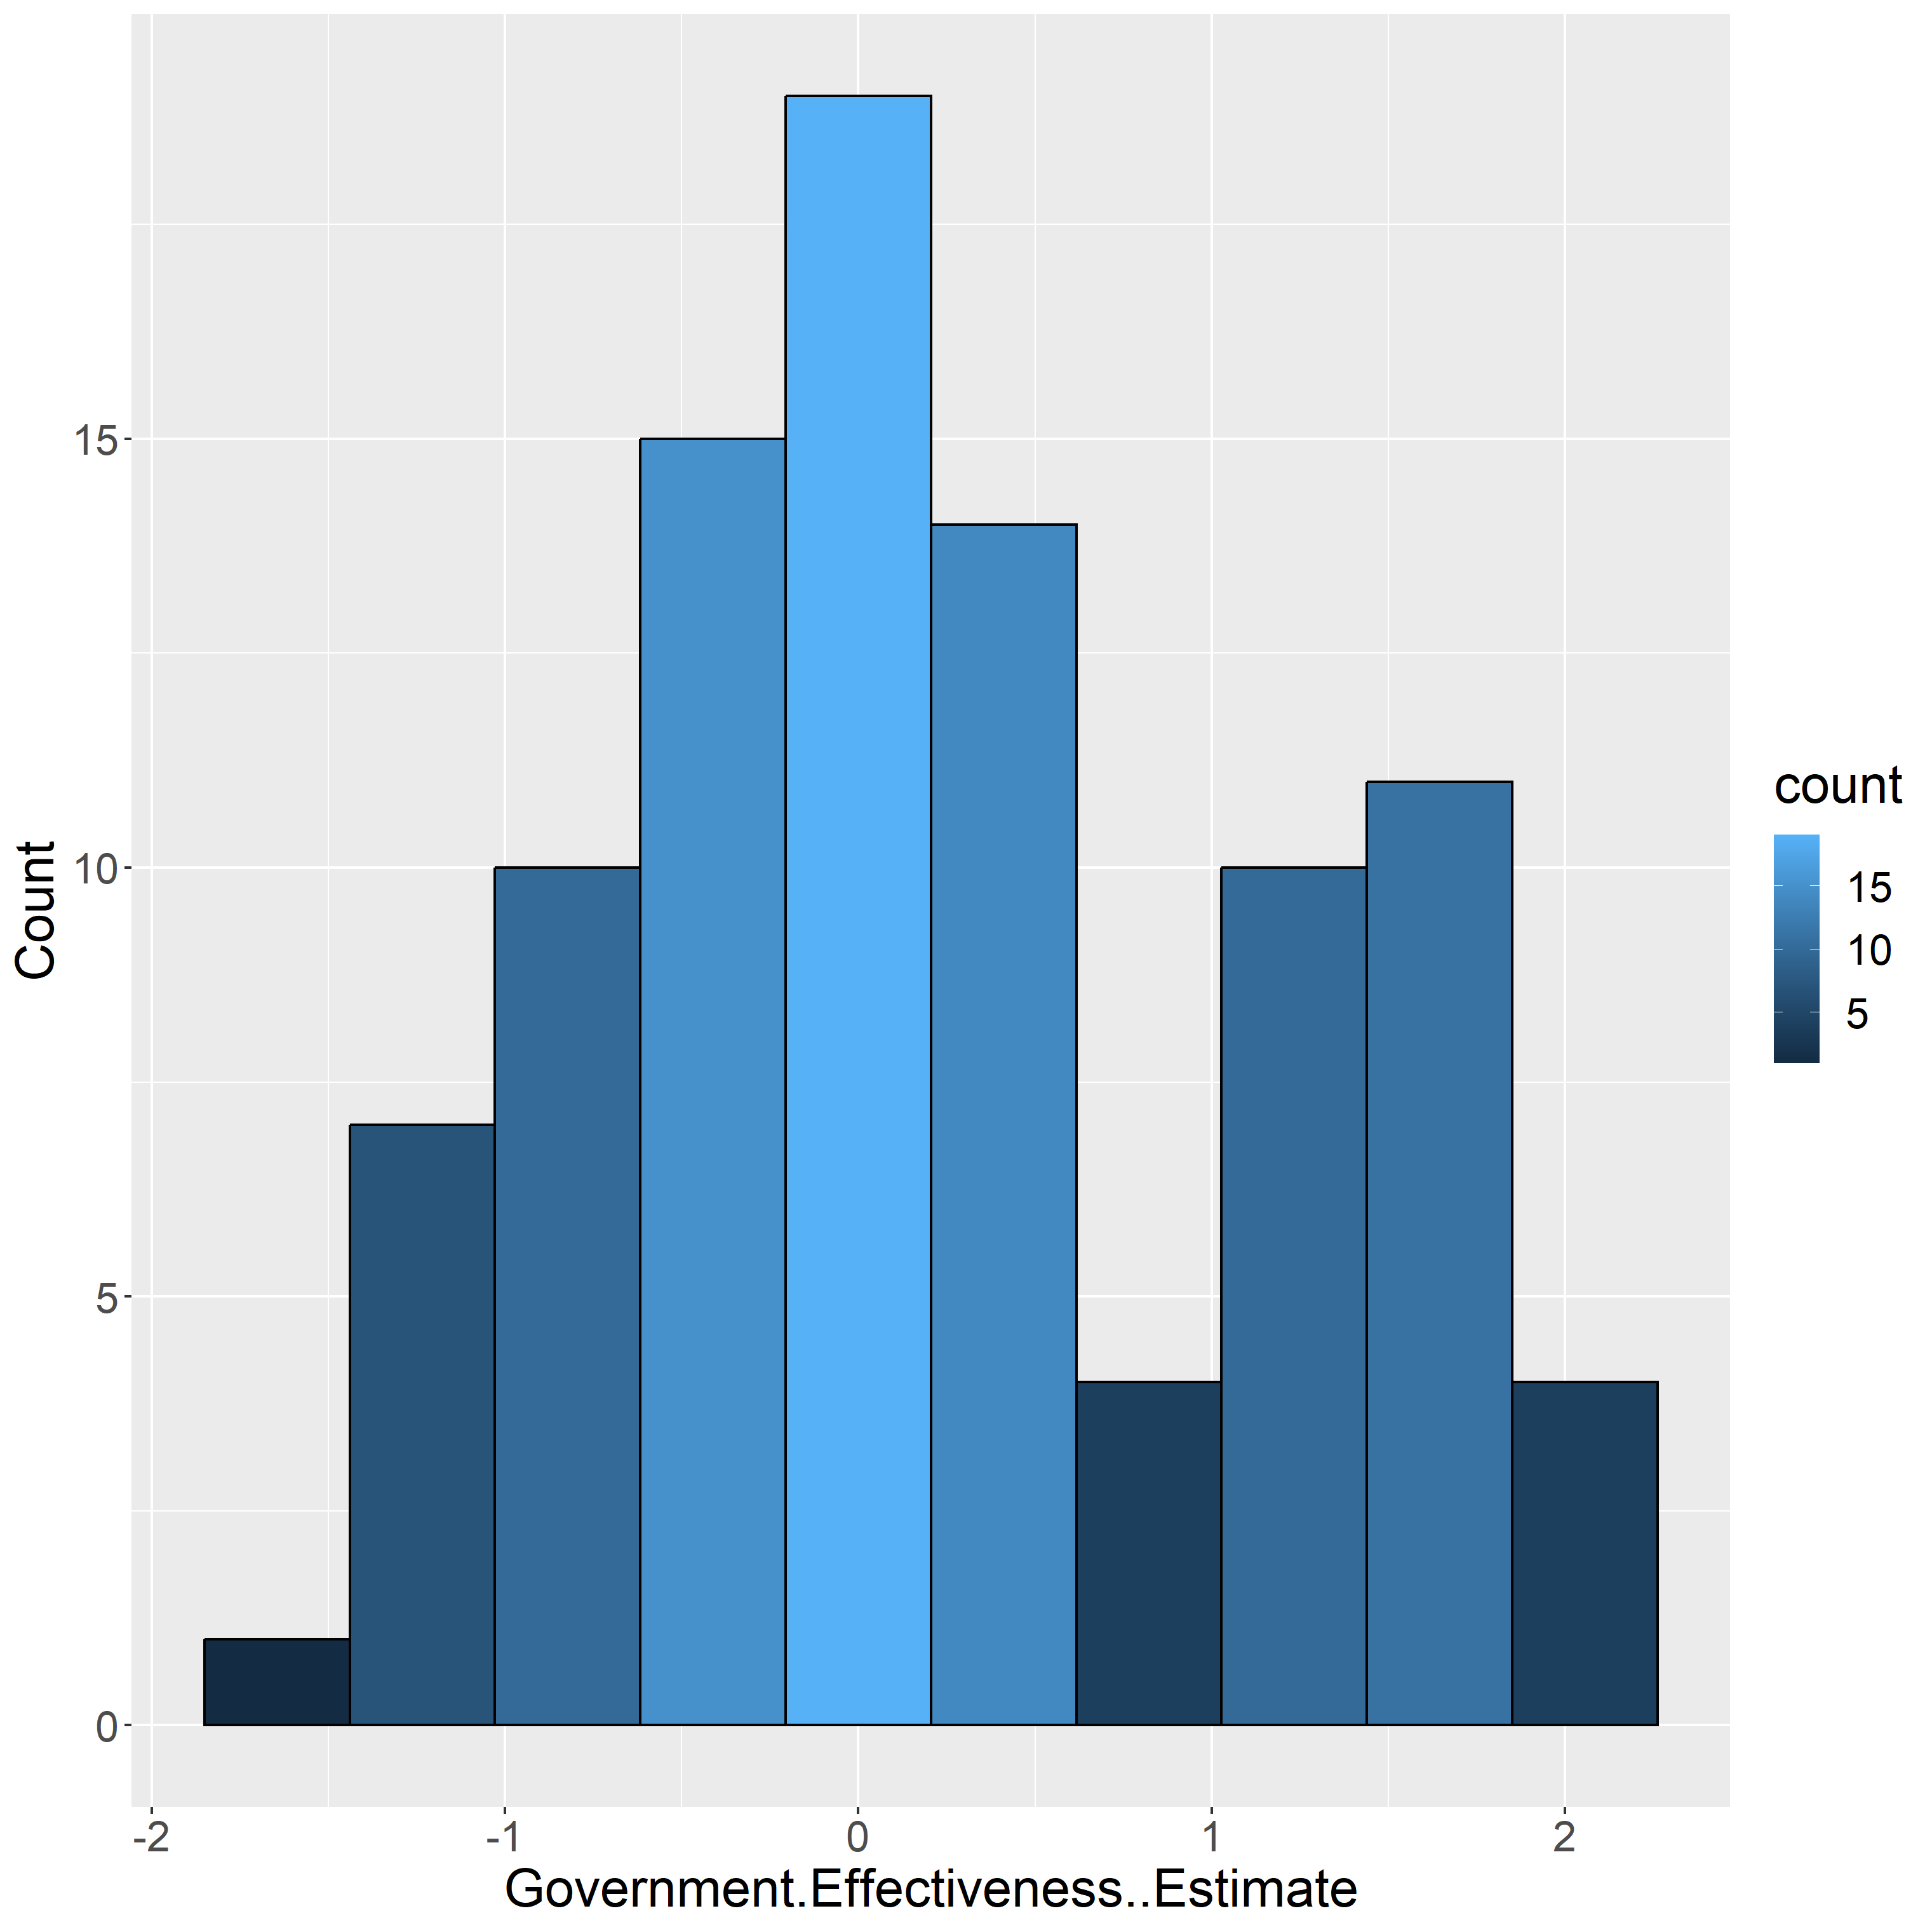
\includegraphics[width=.32\textwidth]{distribution_Government Effectiveness- Estimate.png}\hfill
		\\[\smallskipamount]
		\hfill
		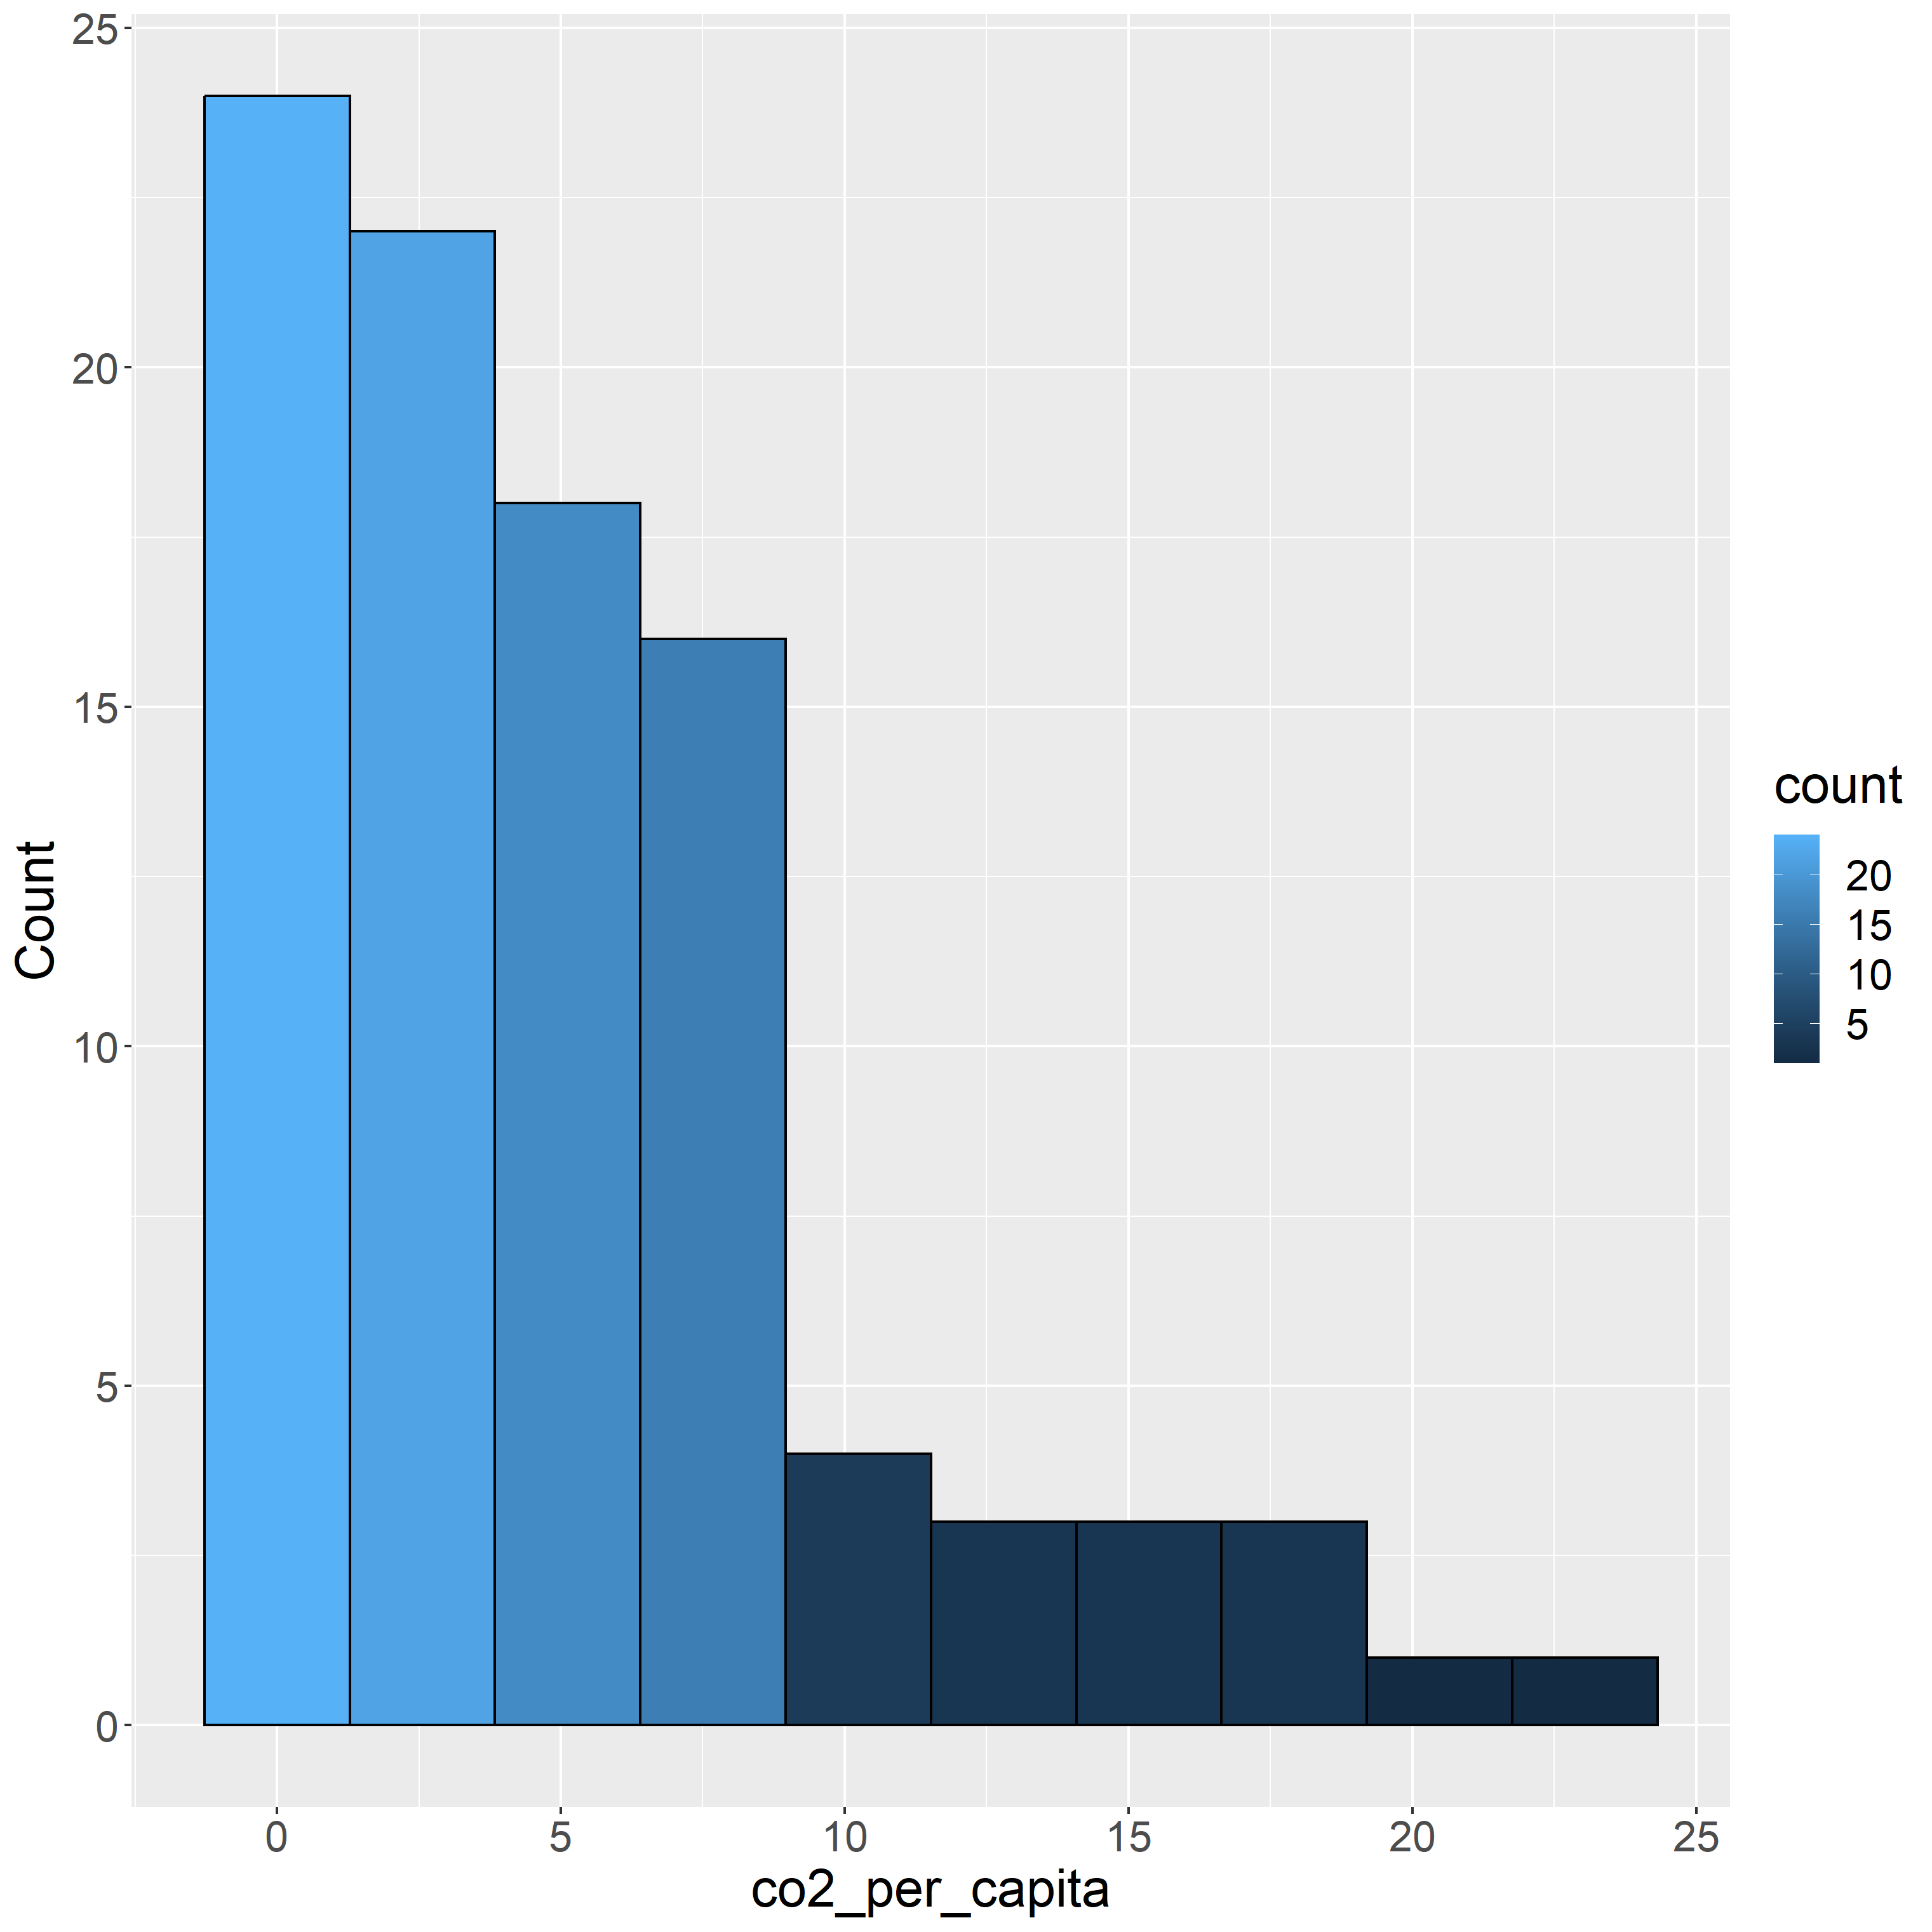
\includegraphics[width=.32\textwidth]{distribution_co2_per_capita.png}\hfill
		\caption{Distributions of the covariates and of the outcome variable \textit{co2\_per\_capita}}\label{fig:covariate_distribution}
	\end{figure}
	
	\section{Regression models}
	
	\subsection{Model 1: Ordinary Linear Regression (OLS) with all covariates}

	We fit an OLS model according to the formula:
	\begin{equation}
		co2\_per\_capita \backsim gdp + [esg\_selected\_indicators]
	\end{equation}
	where the \textit{esg\_selected\_indicators} are the ones listed in Table \ref{table:esg_small_set}.
	\begin{figure} 
		\centering
		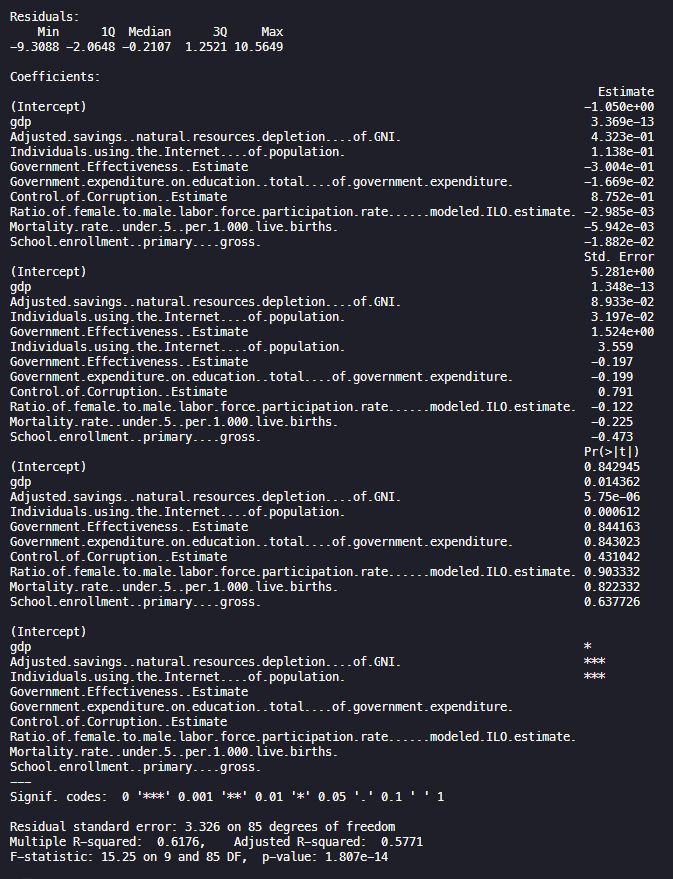
\includegraphics[width=1\linewidth]{summary_mod1.png}
		\caption{\textit{Summary of the Ordinary Linear Regression model (Model 1).}}
		\label{fig:summary_mod1}
	\end{figure}
	The results are shown in the Figure \ref{fig:summary_mod1} and we can see that the adjusted R-squared is , indicating that the covariates are explaining a good portion of the outcome variable. Moreover, the variables \textit{Individuals using the Internet (\% of population)} and \textit{Adjusted savings: natural resources depletion (\% of GNI)} have the lowest p-value, indicating a good correlation with the outcome variable $CO_2\ emission$.

	\paragraph{Residual plot}
	\begin{figure} 
		\centering
		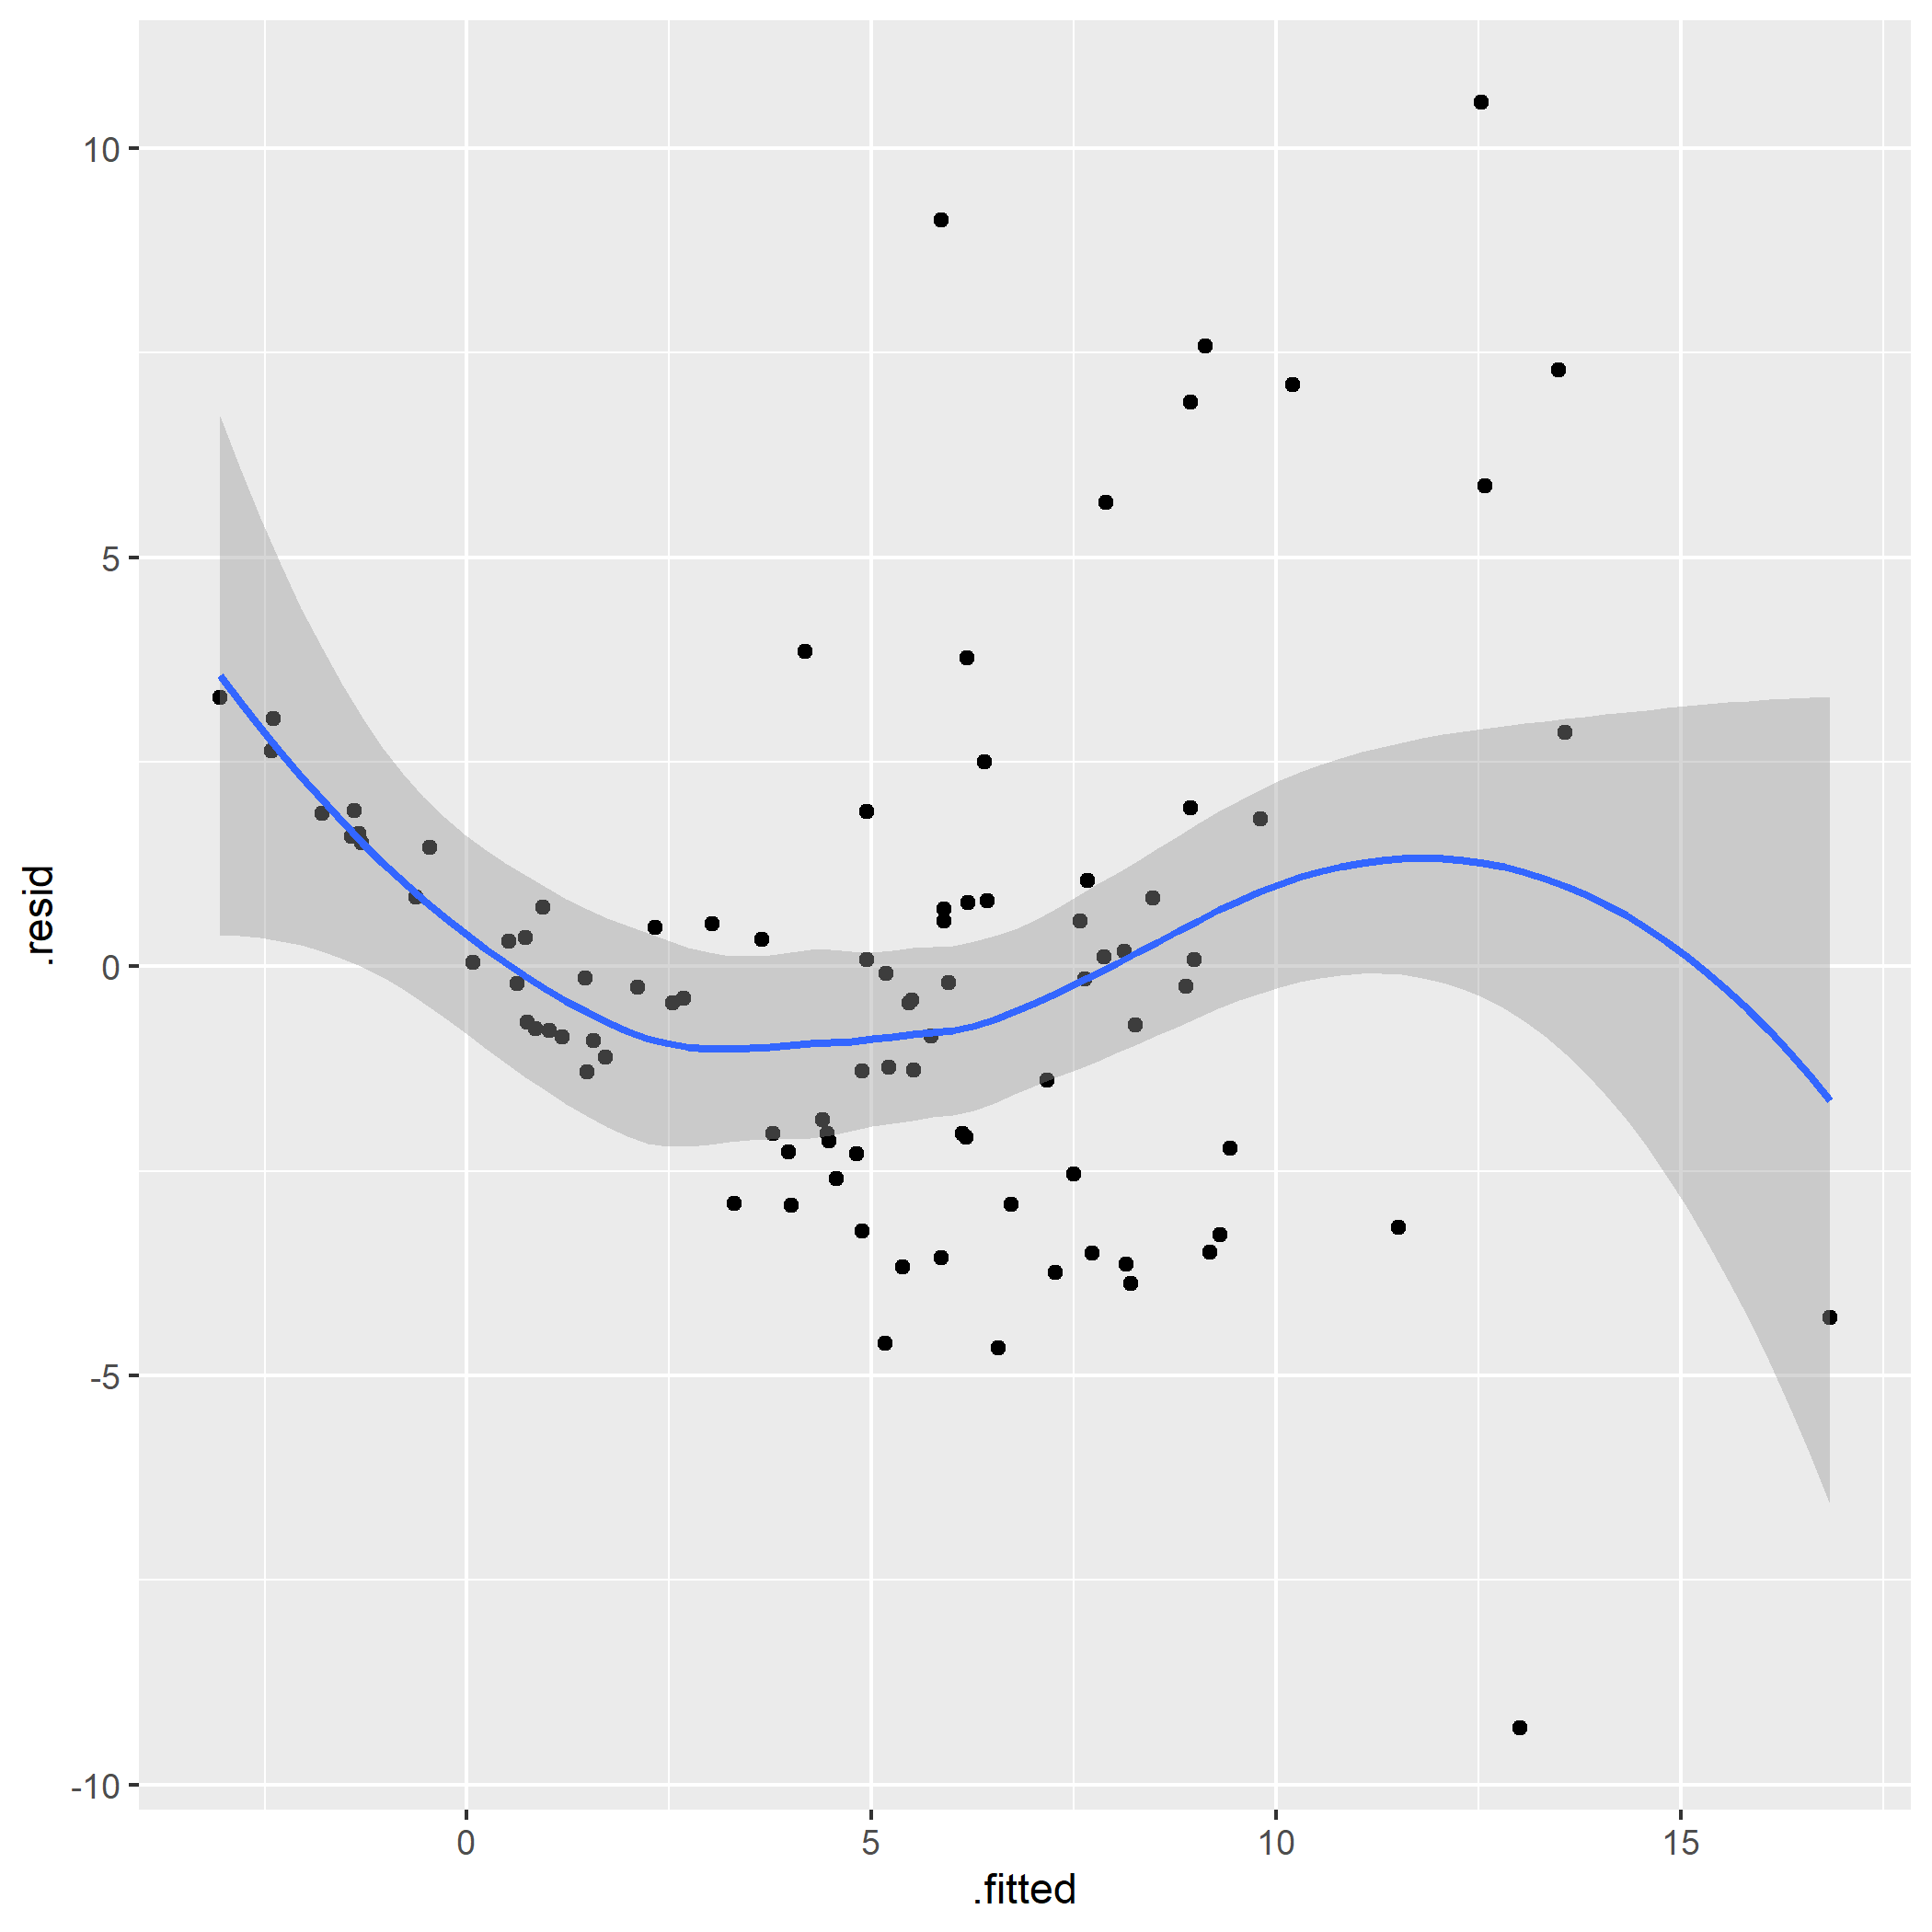
\includegraphics[width=1\linewidth]{residuals_mod1.png}
		\caption{\textit{The plot shows the residual values vs the fitted values for Model 1.}}
		\label{fig:residuals_mod1}
	\end{figure}
	The residual plot is shown in Figure \ref{fig:residuals_mod1} and we see that the errors are not homoskedastic and they have a quadratic shape, so in order to have a fully explanatory linear model and to use it for causal inference, we should fix these issues first.
	
	\subsubsection{Model 2: Most relevant covariates only, with quadratic terms}
	Based on the shape of the residual plot (Figure \ref{fig:residuals_mod1}), we decided to select only the covariates with the lowest p-value, in order to reduce the complexity of the model, while adding few quadratic terms according to the formula:
	\begin{align}
		\nonumber co2\_per\_capita &\backsim \\
		\nonumber &gdp\ *\ Individuals\ using\ the\ Internet\ (\%\ of\ population)\ +\\
		\nonumber &gdp\ *\ Adjusted\ savings:\ natural\ resources\ depletion\ (\%\ of\ GNI)+\\
		\nonumber &(Individuals\ using\ the\ Internet\ (\%\ of\ population) )^2\\ 
		\nonumber &(Adjusted\ savings:\ natural\ resources\ depletion\ (\%\ of\ GNI))^2, 
	\end{align}
	\begin{figure} 
		\centering
		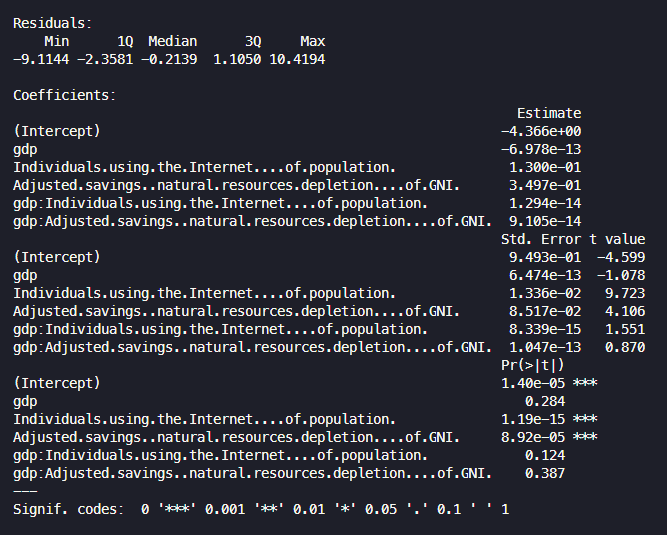
\includegraphics[width=1\linewidth]{summary_mod2.png}
		\caption{\textit{Summary of the Model 2.}}
		\label{fig:summary_mod2}
	\end{figure}
	\begin{figure} 
		\centering
		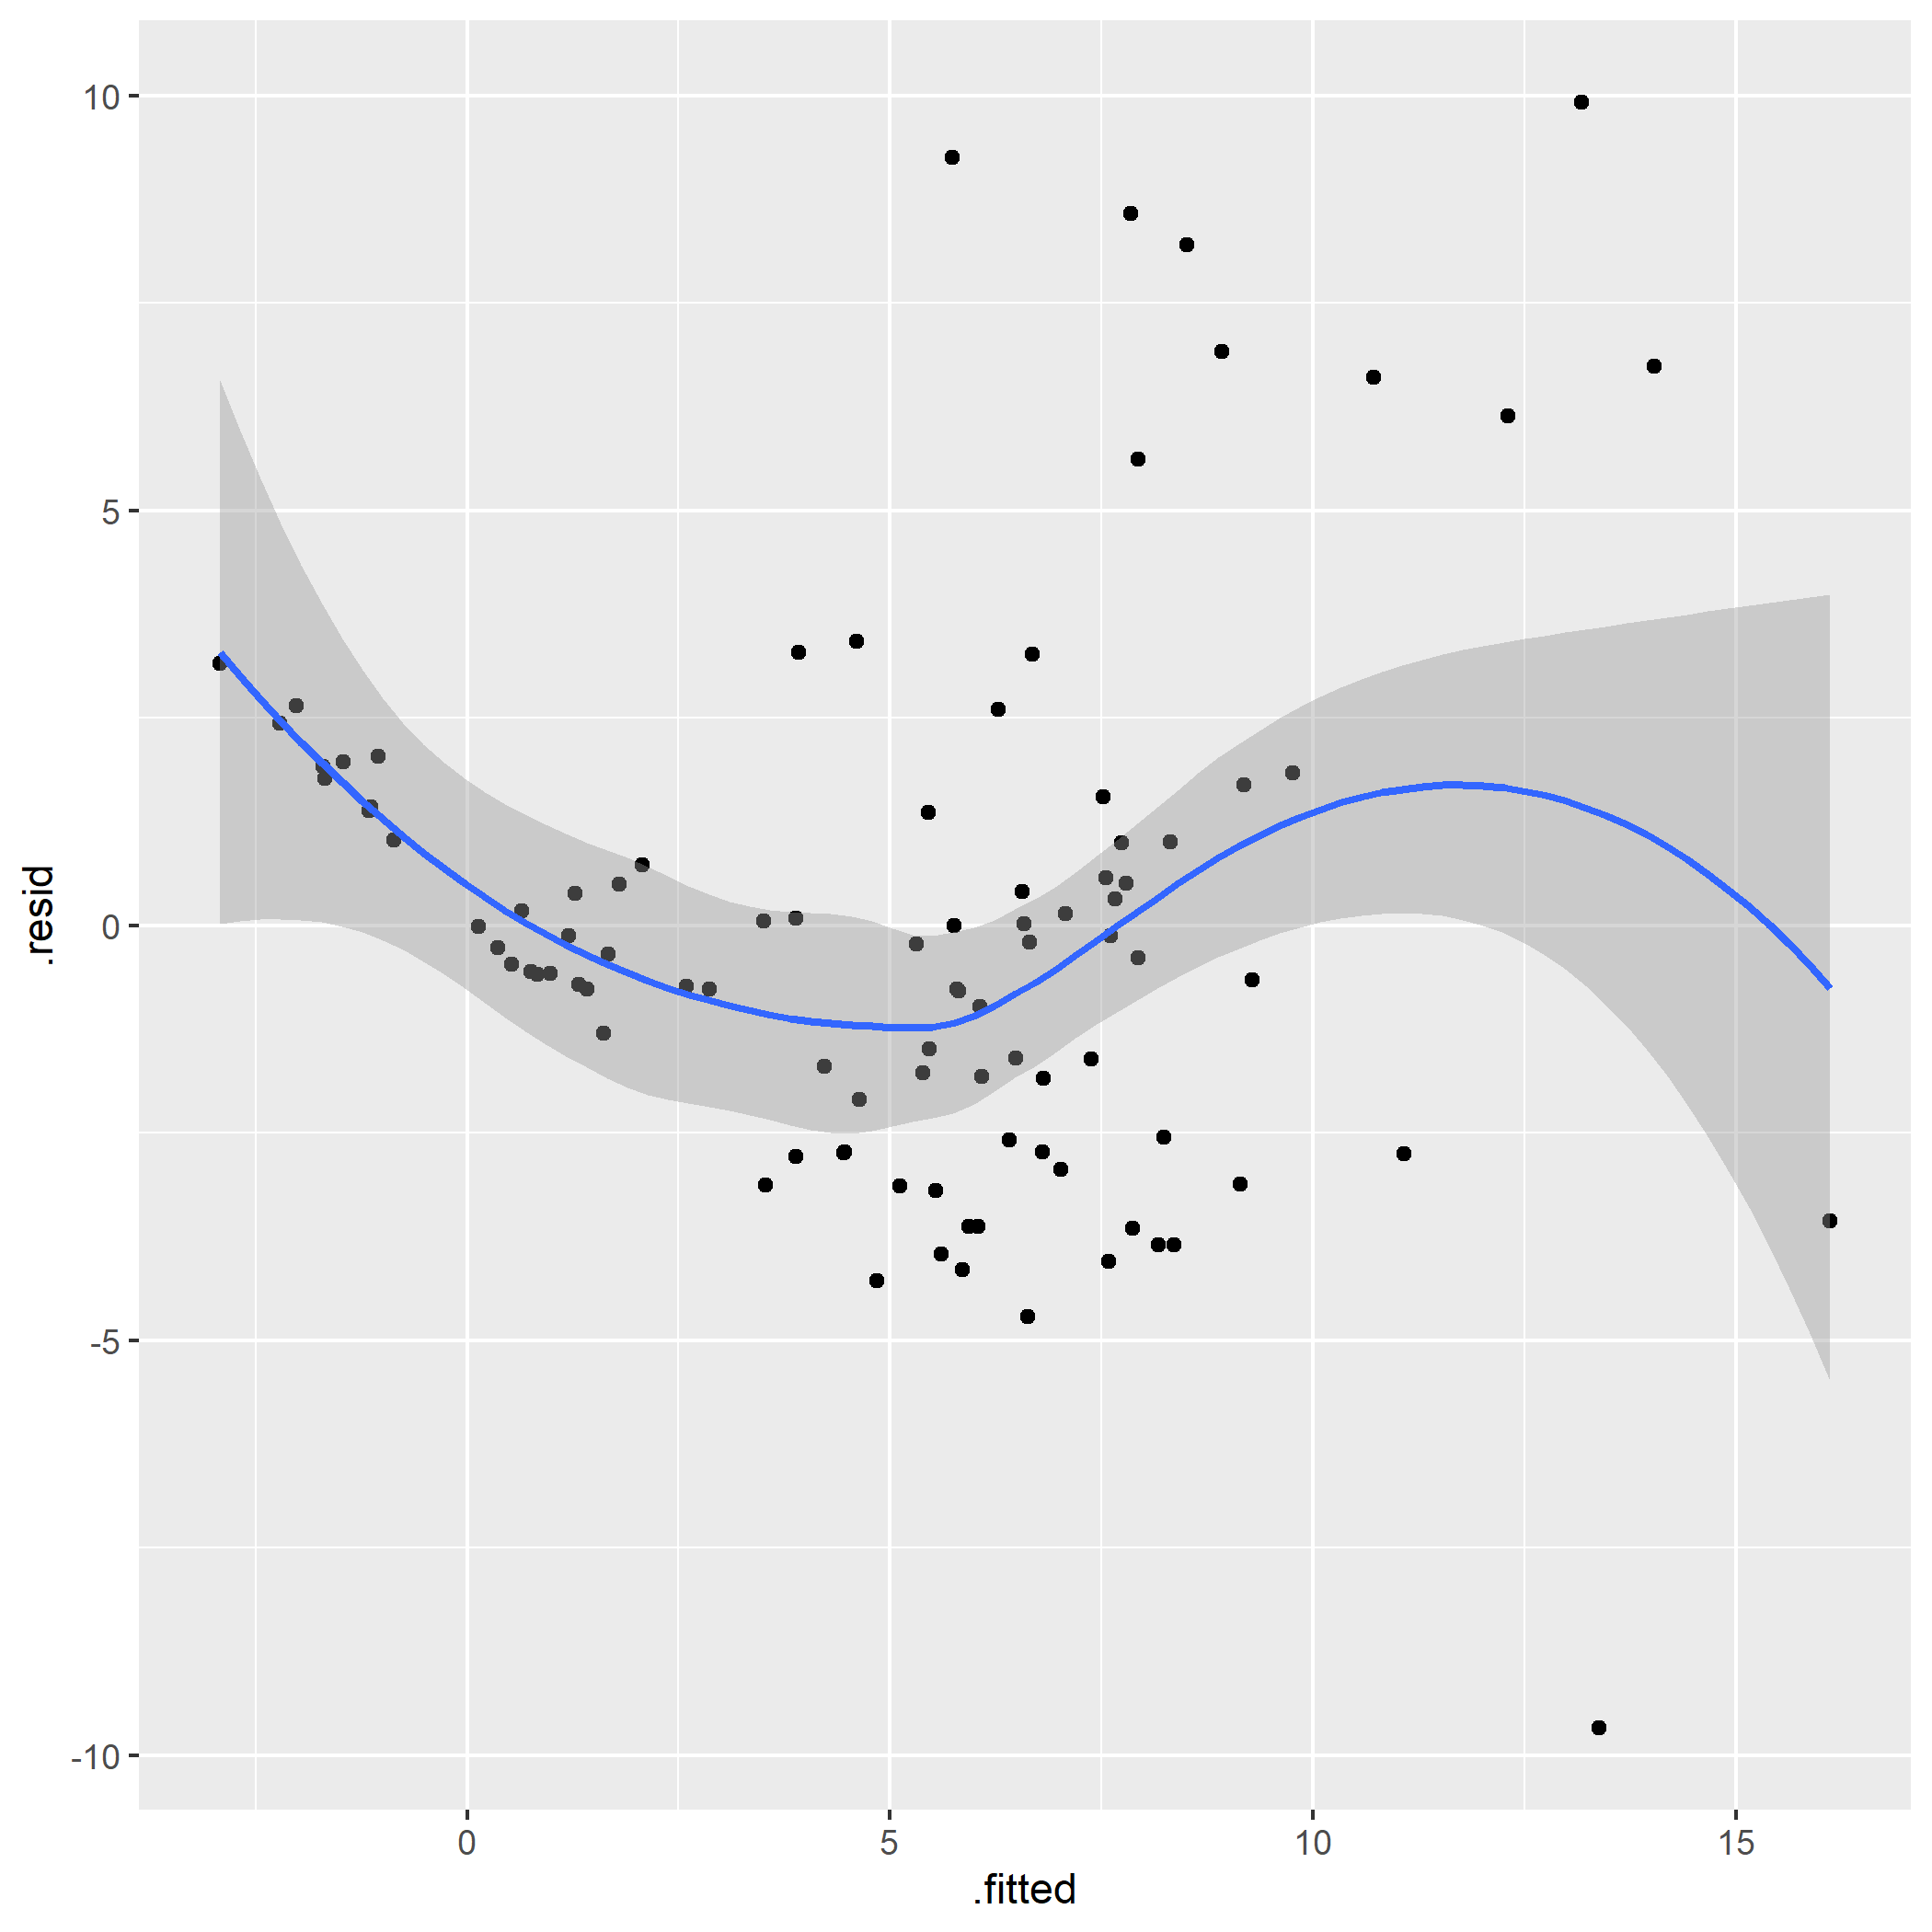
\includegraphics[width=1\linewidth]{residuals_mod2.png}
		\caption{\textit{The plot shows the residual values vs the fitted values for Model 2.}}
		\label{fig:residuals_mod2}
	\end{figure}
	Even though, the \textit{adjusted R-squared} increased (see Figure \ref{fig:summary_mod2}), the residual plot did not change significantly and it highlights the same previous issues (see Figure \ref{fig:residuals_mod2}).
	
	\newpage

	
\end{document}


